\documentclass{rnu-thesis}

\usepackage[protrusion]{microtype}

% --- Algorithms (float + pseudocode)
\usepackage{algorithm}
\usepackage{algpseudocode}

\usepackage{tikz}
\usetikzlibrary{arrows.meta,positioning,shapes.geometric,shapes.symbols,fit,calc,matrix,graphs}
\tikzset{>=Stealth}

% --- Code listings without external deps
\lstset{
  basicstyle=\ttfamily\small,
  numbers=left,
  numbersep=6pt,
  frame=single,
  breaklines=true,
  tabsize=2,
  float=htbp,
  captionpos=t
}

% --- Bibliography via biblatex ---
\usepackage[backend=biber,style=ieee,sorting=nty,maxbibnames=99]{biblatex}
\addbibresource{x_bibliography/references.bib}

% ====== Thesis metadata ======
\setthesisinfoLV
  {Starpplatformu kases un naudas pārvedumu platformas ,,Ethnocount'' projektēšana un izstrāde nelielām valūtas maiņas tīkliem, izmantojot Flutter un Supabase}% LV Title
  {Farruhs Muzrabovs}% LV Student
  {Dr.sc.ing., prof. Jeļena Čaiko}% LV Supervisor
  {42484 Informācijas sistēmas (bak.)}% LV Study programme
  {Dabaszinātņu un datortehnoloģiju katedra}% LV Department
  {2026}% Year

\setthesisinfoEN
  {Design and Implementation of a Cross-Platform Treasury and Money-Transfer Platform (``Ethnocount'') for Small Currency-Exchange Networks Using Flutter and Supabase}% EN Title
  {Farruh Muzrabov}% EN Student
  {Dr.sc.ing., Prof. Jelena Chayko}% EN Supervisor
  {42484 Information Systems (BSc)}% EN Study programme
  {Department of Natural Sciences and Computer Engineering}% EN Department
  {2026}% Year

% ====== Manual thesis scope ======
\setthesisscope
  {74}% Total pages
  {11}% Total tables
  {8}% Total figures
  {0}% Total algorithms
  {12}% Total listings
  {2}% Total annexes
  {20}% Total references

\begin{document}

\input{a_frontmatter/title_page_lv}
\clearpage
\input{a_frontmatter/title_page_en}
\clearpage

\pagenumbering{arabic}

% ===== Abstracts & Keywords =====
\frontmatterpage
\unchapter{Anotācija}

Daudzās bijušās Padomju Savienības valstīs darbojas nelieli biroji, kas maina vienu valūtu pret citu un nosūta naudu uz citām valstīm. Piemēram, ģimene Uzbekistānā var ienākt šādā birojā, lai saņemtu naudu, ko atsūtījis radinieks, kurš strādā Krievijā, un birojs reizi nedēļā norēķinās ar partneru biroju Maskavā. Šādi biroji bieži ir ģimenes uzņēmumi ar filiālēm vairākās pilsētās un valstīs. Tie ikdienā apgroza ievērojamas naudas summas, taču parasti glabā ierakstus papīra žurnālā vai Excel izklājlapā. Tāpēc kļūdas notiek bieži, un viena izlaista rinda var radīt zaudējumu vairāku tūkstošu ASV dolāru apmērā, kura izsekošanai vēlāk nepieciešamas vairākas nedēļas.

Kļūdas notiek tāpēc, ka birojam patiesībā vienlaikus ir jāuztur trīs dažādu veidu uzskaite. Pirmā ir nauda paša biroja kasē un uz paša biroja kartēm. Otrā ir tekošais parāds ar katru partneru biroju ārzemēs, un šis parāds ir jāseko vairākās valūtās vienlaikus, jo vienam un tam pašam partnerim vienlaikus var būt parāds gan Krievijas rubļos, gan Turcijas lirās. Trešā ir pastāvīgo klientu nauda, kas bieži uzkrāj birojā nelielas summas dažādās valūtās. Standarta grāmatvedības programmas visus trīs šos veidus apvieno vienā skaitlī vienā valūtā, un tas tieši slēpj to, kas birojam patiešām jāredz.

Šajā bakalaura darbā ir aprakstīta programma \emph{Ethnocount}, ko autors izstrādājis šīs reālās problēmas risināšanai. Programma strādā uz telefoniem (Android, iPhone) un datoriem (Windows, macOS, Linux) no vienota koda, tāpēc filiāle var lietot to pašu rīku neatkarīgi no tā, vai operators sēž pie galda vai pārvietojas ar telefonu rokā. Programma trīs uzskaites veidus saglabā atsevišķi --- tieši tā, kā tie patiesībā pastāv; tā pareizi summē naudu pat tad, ja vienam partnerim ir parādi trīs dažādās valūtās; un tā nodrošina, ka pārvedumu nevar nejauši saglabāt divreiz, pat ja operators sliktā interneta savienojuma dēļ nospiež pogu divas reizes. Pastāv arī noteikumi par to, kurš ko drīkst darīt: tīkla dibinātājs redz visu, direktors redz visas filiāles, bet parastais darbinieks redz tikai savu filiāli un pirms pagātnes ierakstu maiņas ir jāprasa direktora atļauja.

Autors uzbūvēja sistēmu, rūpīgi pārbaudīja to ar daudziem automātiskiem testiem, izmērīja, cik ātri tā darbojas uz parasta Windows datora un uz vidējas klases Android telefona, un izmēģināja to divas nedēļas kopā ar reālu maiņas biroju. Izmēģinājuma laikā birojs uzturēja gan veco Excel izklājlapu, gan jauno programmu, un katras nedēļas beigās tās tika salīdzinātas. Jaunā programma neradīja nevienu savu kļūdu. Gluži pretēji, tā atrada trīs vecas kļūdas izklājlapā, kuras operators iepriekš nebija pamanījis.

Darbam joprojām ir ierobežojumi, kas tiek godīgi izklāstīti. Programma vēl nepatstāvīgi neielādē valūtas kursus no interneta --- operatoram tie jāievada manuāli. Tā neļauj operatoram saglabāt pārvedumu, kad nav interneta savienojuma --- šādā gadījumā darbība tiek atteikta, jo ar naudu drošāk ir atteikt nekā riskēt ar nepareizu kārtību vēlāk. Un tā tika pārbaudīta vienā birojā divu nedēļu laikā, nevis daudzos birojos vairāku mēnešu garumā. Šie ierobežojumi norāda dabiskus nākamos soļus projekta attīstībai, kas ir uzskaitīti noslēguma nodaļā.

\thesisscopeLV

\textbf{Atslēgvārdi:} starpplatformu mobilā izstrāde, Flutter, BLoC, Supabase, PostgreSQL, Row-Level Security, glabātās procedūras, divkāršā ieraksta grāmatvedība, naudas pārvedumi, ārvalstu valūtas, vairāku filiāļu operācijas, vairāku nomnieku arhitektūra, idempotence.

\frontmatterpage
\unchapter{Abstract}

In many countries of the former Soviet Union there are small offices that exchange one currency for another and send money abroad. A family in Uzbekistan, for example, may walk into such an office to receive money sent by a relative working in Russia, and the office, in turn, settles up with a partner office in Moscow once a week. These offices are often family businesses with branches in several cities and countries. They handle a lot of money every day, but they usually keep their records in a paper notebook or in an Excel spreadsheet. As a result, mistakes happen often, and a single missed line can lead to a loss of several thousand US dollars that takes weeks to find.

The reason mistakes happen is that the office really has to keep three kinds of accounts at the same time. The first is the money in its own cash drawer and on its own bank cards. The second is the running debt with every partner office abroad, and this debt has to be tracked in several currencies at once, because the same partner can owe the office both Russian roubles and Turkish liras at the same time. The third is the money belonging to regular customers, who often keep a small balance with the office in different currencies. Standard accounting programs mix all three of these into one number in one currency, and that hides exactly the things the office needs to see.

This Bachelor's Thesis describes a programme called \emph{Ethnocount}, which the author designed and built to solve this real problem. The programme works on phones (Android, iPhone) and on computers (Windows, macOS, Linux) from the same code, so a branch can use the same tool whether the operator is sitting at a desk or running between clients with a phone in hand. The programme keeps the three kinds of accounts separate, the way they really are; it adds money up correctly even when the same partner has debts in three different currencies; and it makes sure that a transfer cannot be saved twice by accident, even if the operator taps the button twice on a bad internet connection. There are also rules about who can do what: the founder of the network sees everything, a director sees all branches, and a regular employee sees only his or her own branch and has to ask the director's permission before changing past records.

The author built the system, tested it carefully with many automatic tests, measured how fast it works on a normal Windows computer and on a middle-class Android phone, and tried it for two weeks together with a real exchange office. During the trial the office kept both its old Excel spreadsheet and the new programme up to date, and the two were compared at the end of every week. The new programme did not introduce any mistakes of its own. On the contrary, it found three old mistakes in the spreadsheet that the operator had not noticed before.

The work still has limits, which are stated honestly. The programme does not yet download exchange rates from the internet on its own; the operator has to type them in. It does not let the operator save a transfer when there is no internet --- in such a case the action is refused, because for money it is safer to refuse than to risk a wrong order later. And it was tested in one office over two weeks rather than in many offices over many months. These limits point to the natural next steps for the project, which are listed in the closing chapter.

\thesisscopeEN

\textbf{Keywords:} cross-platform mobile development, Flutter, BLoC, Supabase, PostgreSQL, Row-Level Security, stored procedures, double-entry accounting, money transfers, foreign exchange, multi-branch operations, multi-tenant architecture, idempotency.

\frontmatterpage
\unchapter{Key words / Atslēgvārdi}
\begin{tabular}{p{0.45\linewidth}p{0.45\linewidth}}
\textbf{Cross-platform mobile development} & \textbf{Starpplatformu mobilā izstrāde}\\
Flutter framework & Flutter ietvars\\
BLoC state management & BLoC stāvokļa pārvalde\\
Supabase backend & Supabase aizmugure\\
PostgreSQL & PostgreSQL\\
Row-Level Security & Rindas līmeņa drošība\\
Stored procedures (PL/pgSQL) & Glabātās procedūras (PL/pgSQL)\\
Double-entry bookkeeping & Divkāršā ieraksta grāmatvedība\\
Treasury management & Kases pārvaldība\\
Money transfers & Naudas pārvedumi\\
Foreign-exchange operations & Ārvalstu valūtas operācijas\\
Per-currency partner saldo & Partneru saldo pa valūtām\\
Multi-branch operations & Vairāku filiāļu darbība\\
Role-based access control & Lomu balstīta piekļuves kontrole\\
Approval workflow & Apstiprināšanas darbplūsma\\
Idempotent transactions & Idempotentas transakcijas\\
Clean Architecture & Tīrā arhitektūra\\
Design Science Research & Dizaina zinātnes pētījumi\\
\end{tabular}
\clearpage


% ===== Table of Contents (and optional lists) =====
\tableofcontents

\clearpage
\begingroup\let\addcontentsline\relax\listoffigures\endgroup

\clearpage
\begingroup\let\addcontentsline\relax\listoftables\endgroup

\clearpage
\begingroup\let\addcontentsline\relax\listofalgorithms\endgroup

\clearpage
\begingroup\let\addcontentsline\relax\lstlistoflistings\endgroup
\clearpage

% ===== Chapters =====
\unchapter{Introduction}

\noindent\textbf{Topicality of the problem.}
Cross-border remittances handled by small currency-exchange offices form a sector that hardly anyone outside the trade thinks about, and yet it moves a non-trivial share of the labour-migrant economy of the post-Soviet space. The World Bank's \emph{Migration and Remittances Factbook} repeatedly placed countries such as Uzbekistan, Kyrgyzstan and Tajikistan among the world's top recipients of remittances measured as a share of gross domestic product \cite{ratha2016}, and a sizeable portion of that flow does not pass through retail banks at all --- it travels along chains of family-run exchange offices that settle with each other through informal partner networks. The operational tools available to those offices have remained, in practice, two: a paper journal and a Microsoft Excel spreadsheet. Off-the-shelf accounting software either presumes a trained bookkeeper at the keyboard or hides the multi-currency reality of the business behind a single \emph{base-currency} ledger, which is precisely what the operator does not want to see. The result is a sector that is conspicuously under-served by software, despite handling sums measured in millions of US dollars per branch per year, and despite operating under a risk profile (cash, foreign-exchange, counterparty) that makes the absence of audit-grade records genuinely dangerous. This is the gap that the present thesis sets out to address.

\paragraph{Aim of the study.}
The aim of the work is to design, implement and evaluate a production-grade, cross-platform treasury and money-transfer platform --- \emph{Ethnocount} --- tailored to small multi-branch currency-exchange networks, built on Flutter (client) and Supabase (backend), and demonstrably capable of replacing the spreadsheet-and-paper workflow for the daily operations of a representative operator.

\paragraph{Object of the study.}
The object of the study is the daily operational workflow of a small multi-branch currency-exchange network: the recording of own-branch cash and card movements, the issuing and receiving of cross-border money transfers through intermediary partner offices, the maintenance of per-currency running debt with each such partner, and the bookkeeping of recurring-client multi-currency wallets.

\paragraph{Subject of the study.}
The subject of the study is the design and implementation of a cross-platform information system that supports this workflow, expressed as a Flutter client (with the BLoC state-management pattern, GoRouter, get\_it dependency injection and Hive local cache) on top of a Supabase backend (PostgreSQL~16, Row-Level Security, PL/pgSQL stored procedures and Realtime), under a Clean Architecture discipline and a role-based authorisation model with Creator, Director and Accountant roles.

\paragraph{Research problem.}
The research problem can be stated as follows: there is no off-the-shelf or published open-source system that simultaneously (i)~preserves the three balance domains characteristic of the trade --- own-branch funds, partner saldo, client wallet --- without collapsing them into a single base-currency ledger; (ii)~guarantees the atomic, idempotent creation of multi-table transfers under concurrent and intermittent network conditions; and (iii)~implements a role-based authorisation model that lets branch accountants do their job while preventing them from modifying records outside their assigned branches except through an explicit Director-mediated approval workflow.

\paragraph{Tasks of the study.}
The aim is decomposed into the following tasks:
\begin{enumerate}
  \item to review the relevant literature on double-entry bookkeeping in software, multi-user financial applications, cross-platform mobile frameworks and Backend-as-a-Service platforms, and to articulate the research gap in operational terms (Chapter~1);
  \item to formalise the methodological framing of the work within Design Science Research and to describe the data sources used to elicit requirements (Chapter~1);
  \item to derive the functional and non-functional requirements from interviews and observation of an operating exchange network, and to design the eight-entity domain model around the three-balance-domain principle (Chapter~2);
  \item to specify the PostgreSQL schema and the Row-Level Security policy set, together with the Director-mediated approval workflow that protects multi-branch integrity (Chapter~2);
  \item to implement the platform on Flutter and Supabase, including the idempotent atomic transfer engine, the per-currency partner-saldo subsystem and the dark-fintech design language (Chapter~3);
  \item to evaluate the platform through unit, widget and integration tests, controlled performance measurements and a parallel-use trial with a real operator, and to honestly state the remaining limitations (Chapter~3).
\end{enumerate}

\paragraph{Hypothesis.}
Combining Flutter (with the BLoC pattern) as the cross-platform user-interface layer and Supabase (PostgreSQL with Row-Level Security and stored procedures) as the backend permits the implementation of a three-balance-domain treasury platform that, on the workload of a small multi-branch exchange operator, is (i)~free of the reconciliation errors observed in the prior spreadsheet workflow, (ii)~responsive at sub-300-millisecond median interaction latency on commodity hardware, and (iii)~maintainable by a single developer across a multi-month evolution cycle.

\paragraph{Research methods.}
The work uses systematic literature analysis, semi-structured stakeholder interviews and structured observation of the existing workflow, comparative analysis of candidate frameworks, system design under Clean Architecture and Domain-Driven Design vocabulary, software engineering on Flutter and PL/pgSQL, integration testing of stored procedures against a dedicated Supabase staging environment, instrumented performance measurement on Windows desktop and mid-range Android hardware, and a two-week parallel-use acceptance trial with the target operator.

\paragraph{Scientific novelty.}
Three contributions follow from the work. The first is an explicit, relationally expressed three-balance-domain accounting model with per-currency partner saldo --- a model that, to the best of the author's knowledge, has not been published in this shape and that resolves a real reconciliation pathology of the spreadsheet workflow. The second is a Director-mediated approval primitive that captures a before--after snapshot of every Accountant-initiated edit at request time, allowing the Director to compare states explicitly rather than rely on after-the-fact audit logs. The third is the demonstration that a single developer, using Flutter + BLoC + Supabase, can carry a treasury platform of non-trivial scope (15 tables, 66 migrations, approximately 70\,000 lines of Dart) from concept to a working, operator-accepted system within the time-frame of a Bachelor's thesis.

\paragraph{Approbation of the study.}
The complete source code of the platform is publicly released under a permissive open-source licence at \url{https://github.com/farruhsho/ethnocount} for academic review and independent inspection of the architectural and engineering claims made in this thesis.

\paragraph{Task--chapter mapping.}
The six tasks listed above map onto the three substantive chapters of the thesis as shown in Table~\ref{tab:taskmap}.

{\singlespacing
\begin{table}[h]
  \caption{Mapping of research tasks to thesis chapters}
  \label{tab:taskmap}
  \centering
  \begin{tabular}{ll}
    \toprule
    \textbf{Task}                                                  & \textbf{Chapter}\\
    \midrule
    1. Review literature and articulate the research gap          & Chapter~1\\
    2. Frame the work within Design Science Research              & Chapter~1\\
    3. Elicit requirements and design the three-domain model      & Chapter~2\\
    4. Specify the PostgreSQL schema and the RLS policy set       & Chapter~2\\
    5. Implement the platform on Flutter and Supabase             & Chapter~3\\
    6. Evaluate the platform and state the remaining limitations  & Chapter~3\\
    \bottomrule
  \end{tabular}
\end{table}
}


\chapter{Domain Context, Literature Review and Research Methodology}
\label{chap:litreview}

This chapter does three things. It paints the operational picture of the trade the platform is built for, so that the engineering decisions of the later chapters can be read in context. It then surveys the literature the work is built on, grouped around the four themes most relevant to the task at hand --- double-entry bookkeeping inside software, multi-user financial applications, cross-platform mobile frameworks and Backend-as-a-Service platforms. It closes by stating the research methodology, naming the research gap and listing the criteria against which the work is judged.

\section{The Operational Picture of a Small Currency-Exchange Network}
\label{sec:domain}

Small currency-exchange offices in the post-Soviet region are usually family businesses with two to a dozen branches scattered across cities and countries. The branch is the working unit: it has a till, a card reader or two, a Wi-Fi connection that occasionally drops, and an operator who deals with walk-in customers in cash. The same office almost invariably also handles inbound and outbound money transfers --- labour migrants sending earnings home, traders settling invoices, parents wiring tuition to children studying abroad. These transfers rarely travel through the SWIFT-and-correspondent-bank channels of retail finance. Instead, they hop along chains of informal \emph{partner} offices in the destination country, settled later through a running ledger that is, in the field, often a piece of paper. The author's pre-thesis interviews touched a network with branches in Uzbekistan, Russia, Kazakhstan, Kyrgyzstan, Turkey, the United Arab Emirates and China, and the same shape repeated everywhere: one branch issues a transfer in cash; a partner abroad pays the recipient in another currency; the two offices each adjust their running saldo with each other, in the currency of the transfer, with a dealer-mode rate that captures the spread that is, in practice, the operator's profit.

A single transaction touches three accounting layers at once. The first is the operator's own till and card balances --- the cash that physically lives in the branch and the funds available on the operator's settlement card. The second is the partner saldo: a running debt with the partner office, denominated, crucially, in several currencies simultaneously, because the same partner may receive a payout in Russian roubles today and a payout in Turkish liras tomorrow. The third is the recurring client's wallet, where a long-standing customer may keep a positive balance in dollars and a different positive balance in dirhams, drawn down as transfers are dispatched. Off-the-shelf software --- 1C, QuickBooks, Wave --- collapses these three layers into a single, single-currency ledger and absorbs the foreign-exchange differences into a generic \emph{exchange rate variation} account. For a business whose entire revenue model is the spread between currencies, this collapse hides the very signal the operator needs to see.

The errors that emerge from this mismatch are not theoretical. During the requirements-elicitation phase of the project, the operator described several incidents in which a missing column in the spreadsheet, an unsigned partner adjustment, or a transfer recorded twice because of a flaky connection on the operator's phone, produced a multi-thousand-US-dollar discrepancy that took weeks of forensic scrolling to reconcile. One of these incidents directly motivated the introduction of the idempotency key on transfer creation described in Chapter~\ref{chap:implementation}; another motivated the dedicated approval workflow on Accountant edits described in Chapter~\ref{chap:methodology}.

A second feature of the trade that shaped the design is its role structure. A typical network has a Creator (the founder, who owns the data and the credentials), one or more Directors (trusted managers who can see across all branches) and Accountants attached to specific branches (operators who run the day-to-day work but whose access to other branches' data is restricted). Sensitive operations such as deleting a transfer or modifying a client record cannot be left at the Accountant's discretion without compromising audit trails; equally, requiring the Director to log in for every correction would paralyse the workflow. The natural answer is a two-step protocol in which the Accountant \emph{proposes} a change, the system captures the before-state, and the Director approves or rejects from a single screen. This is the approval workflow that section~\ref{sec:approval} formalises and that Chapter~\ref{chap:implementation} implements as a PL/pgSQL RPC.

\section{Double-Entry Bookkeeping in Software Systems}
\label{sec:doubleentry}

Double-entry bookkeeping is rarely cited in computer-science papers, but it is the silent backbone of nearly every accounting system in commercial use. The convention, codified in print by Luca Pacioli in 1494 \cite{pacioli1494} but considerably older in practice, records every economic event as two equal and opposite entries: a debit on one account, a credit on another, summing to zero. The invariant is mechanical, which is precisely the point --- a third party can detect arithmetic errors in a ledger by simple summation, without needing to understand the business it describes. The discipline survives in modern software, although the paired entries are usually generated automatically and hidden from the user interface.

In the software-engineering literature the relevance of double-entry has been argued repeatedly. Fowler, in \emph{Patterns of Enterprise Application Architecture}, names the \emph{Accounting Transaction} pattern as a near-universal building block for financial systems and warns explicitly against the naive shortcut of updating two balance rows in sequence without a wrapping transactional boundary \cite{fowler2002}. The warning is borne out in practice: a sizeable share of the financial-software incidents documented in industrial post-mortems trace back to this exact failure mode, a row updated and the program crashed before the matching row was touched. Event-sourcing literature generalises the discipline further: each business event is recorded as an immutable fact in an append-only log, and balance views are derived as projections \cite{wesner2018,fowler2017event}. The approach has the secondary virtue of producing an audit trail by construction.

The platform described in this thesis adopts a hybrid posture. The fundamental store is an append-only \texttt{ledger\_entries} table in PostgreSQL, mirroring the event-sourcing tradition; balance rows are kept denormalised in dedicated tables for fast lookup. The atomicity of the dual write is enforced at the database layer through stored procedures that wrap both writes inside an implicit transaction, so that the schema preserves the double-entry invariant by construction rather than by trust in the application layer.

\section{Multi-User Financial Applications: A Brief State of the Art}
\label{sec:soa}

A review of consumer-facing mobile applications for shared finances exposes a sharp bifurcation. At one end sit informal expense-splitters --- Splitwise being the canonical example --- which prioritise frictionless peer-to-peer reconciliation among friends and intentionally avoid currency-level rigour \cite{splitwise2024}. At the other end sit small-business accounting suites such as Wave, Zoho Books and QuickBooks, which implement formal double-entry but presume a stable single-currency operating environment and a trained bookkeeper at the keyboard \cite{quickbooks2024}. Between these two extremes the academic literature on cross-border remittance networks, in particular the World Bank \emph{Migration and Remittances Factbook} series \cite{ratha2016}, documents the operational practices of intermediary settlement networks but does not produce a generalised software framework for them.

Enterprise treasury management systems --- SAP Treasury, Kyriba \cite{kyriba2023} --- do cover the multi-currency multi-branch scenario natively, but they are priced and scoped for organisations several orders of magnitude larger than the target of this work, and their adoption curve is the territory of trained corporate treasury teams, not branch operators. The niche the present platform aims at therefore sits in a genuinely unoccupied region of the design space: small (two to a dozen branches), multi-currency, multi-tenant by role rather than by company, designed to be used by branch personnel under time pressure with walk-in clients waiting at the counter.

Table~\ref{tab:soa} compares the platforms reviewed in this section along the dimensions that mattered for the gap analysis: collaboration model, multi-currency support, partner-mediated transfer support, role-based authorisation and target operator profile.

{\singlespacing
\begin{table}[h]
  \caption{Representative existing systems compared against the niche of this thesis}
  \label{tab:soa}
  \centering
  \begin{tabular}{lcccc}
    \toprule
    \textbf{System}      & \textbf{Multi-cur.} & \textbf{Partner saldo} & \textbf{Role-based} & \textbf{Target}\\
    \midrule
    Splitwise            & limited             & ---                    & ---                  & peers\\
    Wave / Zoho Books    & limited             & ---                    & partial              & small biz\\
    QuickBooks           & yes (collapsed)     & ---                    & yes                  & SMEs\\
    1C: Accounting       & yes (collapsed)     & ---                    & yes                  & trained accountant\\
    SAP Treasury, Kyriba & yes                 & yes (corporate)        & yes                  & enterprise\\
    \textbf{Ethnocount}  & \textbf{yes (per-cur.)} & \textbf{yes (per-cur.)} & \textbf{yes} & \textbf{small exchange}\\
    \bottomrule
  \end{tabular}
\end{table}
}

The conclusion is that no surveyed system simultaneously preserves the three-balance-domain accounting model with per-currency partner saldo \emph{and} targets the operational profile of a small exchange network with branch-level Accountants and a Director who oversees them. This is the gap the platform fills.

\section{Cross-Platform Mobile Frameworks}
\label{sec:crossplatform}

Two waves dominate the cross-platform mobile space at the time of writing. The first, exemplified by React Native and Cordova, executes JavaScript through a bridge to native UI components: the developer writes once in a JavaScript dialect, and the framework instantiates platform-native widgets at runtime. The second, represented by Flutter, ships its own rendering engine and draws every pixel itself, so the application looks and behaves identically on every platform at the cost of bundling roughly twenty megabytes of engine code. The trade-offs are well-documented in the literature, including the often-cited comparative study by Heitk{\"o}tter, Hanschke and Majchrzak \cite{heitkotter2013}, which is now slightly dated on specifics but still correct on the underlying axes: developer productivity, platform fidelity, accessibility and the size of the runtime.

For the present project the choice fell on Flutter for three reasons that are pragmatic rather than ideological. The first is that the same Dart codebase targets Android, iOS and the three desktop platforms simultaneously, with Windows in particular non-negotiable: the network's branches run on Windows desktops, and a web-only client was not acceptable. The second is that the Dart language is statically typed with sound null-safety, which catches a meaningful fraction of the bugs that would otherwise surface only in production. The third, more subjective but no less important for a single-developer project, is that Flutter's hot reload --- which redraws the user interface in under a second after a source change --- makes the iterative-incremental development rhythm of section~\ref{sec:dsr} tractable.

Table~\ref{tab:frameworks} compares the candidates considered.

{\singlespacing
\begin{table}[h]
  \caption{Cross-platform mobile frameworks considered at project start}
  \label{tab:frameworks}
  \centering
  \begin{tabular}{lccc}
    \toprule
    \textbf{Dimension}         & \textbf{Flutter} & \textbf{React Native} & \textbf{Kotlin Multipl.}\\
    \midrule
    Android / iOS              & stable           & stable                & stable\\
    Windows desktop            & stable           & experimental          & via shared logic only\\
    macOS / Linux desktop      & stable           & experimental          & limited\\
    Type system                & sound nulls      & TypeScript optional   & sound nulls\\
    Hot reload                 & sub-second       & sub-second            & slower\\
    Single-author velocity     & high             & medium                & medium\\
    Default look on Windows    & matches design   & off                   & native\\
    \bottomrule
  \end{tabular}
\end{table}
}

\section{Backend-as-a-Service Platforms}
\label{sec:baas}

Backend-as-a-Service platforms emerged in the early 2010s as a way for small development teams to skip the operational burden of running their own application servers. Firebase pioneered the category, with a proprietary document store, opinionated security rules and a generous free tier; Supabase, launched in 2020 \cite{copplestone2024}, set itself apart by exposing a full PostgreSQL database directly to the developer rather than a custom document layer. Supabase retains the queryability, the transactional guarantees and the strong type system of PostgreSQL, while wrapping them in managed services for authentication (GoTrue), automatic REST-and-RPC exposure (PostgREST), real-time logical replication over WebSockets (Realtime), object storage and edge functions.

The choice between the two for the present platform was, in the end, not difficult. The business semantics require that the dual write of a transfer (the source debit and the destination credit) be atomic, and the natural way to express atomicity over multiple table writes is a database transaction wrapped in a stored procedure --- not a custom security-rule DSL that cannot easily express cross-document constraints. Firebase Cloud Functions can wrap multiple Firestore writes in a single batched commit, but cross-document transactional behaviour in Firestore is intentionally bounded for scalability reasons \cite{firebase2024}, and the multi-table joins that the reporting screens of the platform rely on (transfers joined with branches joined with counterparties joined with currencies) are awkward to express against a document store. PostgreSQL handles those joins natively in single-millisecond time.

Brewer's CAP theorem \cite{brewer2000} reminds the architect that any distributed system must in the limit choose two out of consistency, availability and partition-tolerance. The platform under discussion prioritises consistency for write operations --- a transfer either succeeds end-to-end or has no visible effect --- and pays for that choice by refusing offline writes (section~\ref{sec:offline}). The decision is appropriate to the domain: a missed read while the network is down is mildly inconvenient; a write that the operator believes succeeded but did not produce a row in \texttt{transfers} would be a financial incident.

\section{Clean Architecture, Domain-Driven Design and the BLoC Pattern}
\label{sec:cleanarch}

The architectural vocabulary of the work is borrowed from two sources. Evans' \emph{Domain-Driven Design} \cite{evans2003} contributes the discipline of treating the business domain as a separately identifiable, pure-Dart core --- entities, value objects, repositories as interfaces --- around which the framework-bound layers orbit. Martin's \emph{Clean Architecture} \cite{martin2017} contributes the layering and the dependency rule: source dependencies point only inward, from outer concrete layers (presentation, data) toward the abstract domain core. The combination is not aesthetic but operational. It makes the domain entities unit-testable in isolation, without a Flutter test environment; it lets the backend (Supabase) be substituted with a mock implementation in tests without touching the BLoCs; and it ensures that when Flutter releases a breaking change in its widget library, the change touches only the presentation layer rather than rippling through the entire codebase.

The presentation layer uses the BLoC (Business Logic Component) pattern \cite{flutter2024bloc}, in which every screen is driven by a small state machine whose inputs are typed \emph{Events} and whose outputs are typed \emph{States}. BLoC was preferred over Provider or Riverpod for two pragmatic reasons. The first is that the explicit Event--State model maps cleanly onto the transactional discipline that financial operations demand: every operator action corresponds to an Event, every visible screen configuration corresponds to a State, and the developer cannot accidentally update part of the screen without producing the matching Event. The second is testability --- events and states are pure values, exercised in isolation through the \texttt{bloc\_test} package, without requiring a widget tree.

\section{Research Methodology}
\label{sec:dsr}

The work is framed within Design Science Research (DSR) as formulated by Hevner, March, Park and Ram \cite{hevner2004}. DSR posits that knowledge in engineering disciplines is produced through the construction of artifacts whose behaviour answers a defined research question. The artifact in this thesis is the Ethnocount platform itself; the knowledge contribution is the documented set of design decisions that allowed the three-balance-domain model to be expressed in a relational schema and operated atomically under the operational and authorisation constraints of the trade.

The DSR cycle used here proceeded through four iterations. In each iteration a focused sub-problem was identified --- per-currency partner saldo in one iteration, the approval workflow in another, the balance-guard triggers in a third, AML/KYC foundations in a fourth --- a candidate design was implemented, the design was evaluated against the criteria stated in the hypothesis, and the lessons learned informed the next iteration. The iterations were not strictly sequential: several earlier decisions were revisited when later iterations exposed their limits. Migration~047 of the production schema, for example, replaced a USD-collapsed partner saldo with the per-currency JSONB model only after iteration three had shown the original collapse to hide real exposure when the same partner had simultaneous debts in three currencies (the trigger event was described by the operator during an interview between iterations two and three).

The day-to-day work inside each iteration followed an iterative-incremental engineering rhythm closer in spirit to disciplined Agile than to ceremonial Scrum. A single developer worked through a backlog organised around vertical slices: every slice delivered a coherent feature end-to-end, from the migration through the stored procedure and the BLoC to the screen the operator would actually use. Slices were kept small enough to keep the trunk continuously deployable, and database migrations were numbered, idempotent SQL files that could be replayed in any environment. Source control was Git; every commit referenced the slice it implemented. Code review was self-administered with the help of the Dart analyser configured for strong null-safety and the Supabase advisor for the database layer. A short handoff document was kept current at all times in case the project needed to be passed to another developer --- a discipline that, although not used in anger, was helpful in surfacing implicit assumptions.

\paragraph{Data sources.}
The functional requirements were elicited from three complementary sources. The first was a series of semi-structured interviews with the operator running the existing spreadsheet workflow, covering the activities of a typical day, the kinds of errors the operator had experienced and the data items currently kept in the operator's head rather than in any artifact. The second source was structured observation: the author sat with the operator across four working sessions, watching the spreadsheet being filled in real time and noting moments of hesitation, rework or branched logic. The third source was the existing spreadsheet itself, treated as a tacit specification --- column names, conditional formats and hand-written notes in the margin were all carefully reverse-engineered into entity attributes.

\paragraph{Evaluation methods.}
The evaluation, reported in Chapter~\ref{chap:implementation}, combines four complementary methods. Automated unit and widget tests verify the correctness of the pure-Dart logic and the rendering of the most safety-critical screens under controlled state. Integration tests against a dedicated Supabase staging project verify the behaviour of stored procedures and Row-Level Security policies, including the atomicity properties claimed in the hypothesis. Performance measurements are taken on a representative Windows desktop and a mid-range Android device, instrumented through chronometers around the most frequent user actions. Finally, a User Acceptance Test was conducted with the operator over two weeks of parallel use, during which both the spreadsheet and the platform were updated with the same operational data and reconciled at the end of each week.

\paragraph{Ethical considerations.}
The interviews and the acceptance trial involved a single business and were conducted under explicit consent. No client-identifying data is included in this thesis; where examples appear, names, phone numbers and account numbers are illustrative placeholders. The codebase contains no hard-coded credentials, and the staging Supabase project used for evaluation was destroyed at the conclusion of the trial. The thesis acknowledges the regulatory complexity of remittance services in some jurisdictions and explicitly limits its scope to the operational dimension of the business rather than its legal one.

\section{Research Gap, Hypothesis and Success Criteria}
\label{sec:gap}

Synthesising the literature reviewed in this chapter with the operational picture of section~\ref{sec:domain}, the research gap can be stated precisely: there is no published or off-the-shelf system that simultaneously (i)~preserves the three-balance-domain accounting model with per-currency partner saldo, (ii)~enforces atomicity and idempotency of multi-table transfer creation through database-level stored procedures rather than application-level checks, and (iii)~combines Row-Level Security with a Director-mediated approval workflow that lets branch Accountants do their work while protecting multi-branch integrity. The hypothesis stated in the Introduction is that a Flutter + BLoC client on a Supabase backend is a sufficient technology stack to close this gap within the engineering envelope of a single bachelor-level developer.

The success criteria against which the rest of the thesis is judged are three. \emph{Correctness} requires that the platform exhibit zero platform-introduced reconciliation errors during the two-week parallel-use trial. \emph{Responsiveness} requires sub-300-millisecond median interaction latency on the reference hardware. \emph{Maintainability} requires that the platform be carried, by a single developer, through a multi-month evolution cycle without irreparable drift between the client and the server schema --- operationalised in this work as: every commit must land on a green build, and every schema change must arrive as a numbered, idempotent migration file.

\section{Chapter Summary}
\label{sec:ch1summary}

The chapter has done four things. It described the operational picture of the small currency-exchange networks the platform is built for, with its three accounting layers, its Creator/Director/Accountant role structure and its tolerance for hand-held devices on flaky networks. It surveyed the literature relevant to the engineering task --- double-entry bookkeeping in software, multi-user financial applications, cross-platform frameworks, Backend-as-a-Service platforms, and the architectural vocabulary of Clean Architecture, Domain-Driven Design and the BLoC pattern. It framed the work within Design Science Research, described the iterative-incremental development rhythm and the four data sources used for requirements elicitation. And it formalised the research gap and the three success criteria against which the rest of the work is assessed.

\noindent\textbf{Conclusions for Chapter~1.}
No surveyed system simultaneously preserves the three-balance-domain accounting model with per-currency partner saldo, enforces atomicity through database stored procedures, and combines Row-Level Security with a Director-mediated approval workflow. The hypothesis is that the combination of Flutter (with BLoC) and Supabase (PostgreSQL with RLS and stored procedures) is sufficient to close this gap inside the engineering envelope of a single bachelor-level developer. The next chapter derives the requirements, designs the domain model and specifies the database schema and the RLS policy set against which that hypothesis will be tested.

\chapter{System Analysis and Architecture Design}
\label{chap:methodology}

The previous chapter framed the problem and the research methodology. The present chapter turns the abstract gap into a system. It begins with the catalogue of functional and non-functional requirements derived from the elicitation activities of section~\ref{sec:dsr}; it proceeds through the domain model, the Clean Architecture pattern, the PostgreSQL schema and the Row-Level Security policy set; and it closes with the design of the Director-mediated approval workflow that turns out to be the central authorisation primitive of the platform.

\section{Functional and Non-Functional Requirements}
\label{sec:requirements}

\subsection{Functional requirements}
\label{ssec:func}

The functional requirements were derived from the three data sources of section~\ref{sec:dsr} --- the operator interviews, the four working-session observations and the existing spreadsheet treated as a tacit specification --- and refined across the four iterations of the DSR cycle. Table~\ref{tab:func} lists the principal requirements with stable identifiers that are referenced from the implementation chapter.

{\singlespacing
\begin{longtable}{p{1.3cm}p{12.5cm}}
  \caption{Functional requirements (principal items)}
  \label{tab:func}\\
  \toprule
  \textbf{ID}  & \textbf{Requirement}\\
  \midrule
  \endfirsthead
  \toprule
  \textbf{ID}  & \textbf{Requirement}\\
  \midrule
  \endhead
  \bottomrule
  \endfoot
  FR-01 & The system shall authenticate users by email and password and load their role and assigned-branches list immediately after sign-in.\\
  FR-02 & The system shall present, on a dashboard, the per-currency balances of every branch the user is authorised to see.\\
  FR-03 & The system shall let an authorised user create a money transfer in one of three modes: own-branch only; partner-mediated (the transfer travels through an intermediary partner); and dealer mode (with explicit buy/sell rates for the spread).\\
  FR-04 & The system shall accept an idempotency key on every transfer-creation request and reject any duplicate request carrying the same key.\\
  FR-05 & The system shall maintain a per-currency running saldo with every intermediary partner, updated atomically whenever a partner-mediated transfer is created or detached.\\
  FR-06 & The system shall maintain a per-client multi-currency wallet (ClientBalance) and shall record every wallet movement as an immutable ledger entry.\\
  FR-07 & The system shall allow the Creator and the Director to administer the catalogues of branches, branch accounts, partners, clients, commissions and exchange rates.\\
  FR-08 & The system shall restrict an Accountant's visibility to the branches listed in the user's assigned-branch-ids attribute.\\
  FR-09 & The system shall route Accountant-initiated modifications of transfers, clients or accounts through a pending-approvals workflow that captures a before-snapshot of the affected row.\\
  FR-10 & The system shall present the Director with a single screen on which the before- and after- states of each pending approval are visible side by side, and on which the Director can approve or reject.\\
  FR-11 & The system shall send real-time notifications to relevant users when a transfer is created, modified, deleted or approved/rejected.\\
  FR-12 & The system shall log every modification of a sensitive entity (transfer, client, account, partner) to an audit trail that records the actor, the timestamp and the before/after states.\\
  FR-13 & The system shall produce per-currency reconciliation reports between the operator's book and the partner's book over a chosen period.\\
\end{longtable}
}

\subsection{Non-functional requirements}
\label{ssec:nonfunc}

The non-functional requirements (Table~\ref{tab:nonfunc}) translate the hypothesis of section~\ref{sec:gap} into measurable engineering targets. They are referenced again in the evaluation section of Chapter~\ref{chap:implementation}.

{\singlespacing
\begin{table}[h]
  \caption{Non-functional requirements}
  \label{tab:nonfunc}
  \centering
  \begin{tabular}{p{1.3cm}p{6cm}p{6cm}}
    \toprule
    \textbf{ID}  & \textbf{Property}        & \textbf{Target}\\
    \midrule
    NFR-01 & Median interaction latency      & $\leq$ 300\,ms on reference hardware\\
    NFR-02 & Cross-tenant data leakage       & Zero rows under integration tests\\
    NFR-03 & Atomicity of transfer creation  & All-or-nothing across all affected tables\\
    NFR-04 & Idempotency of write operations & Server rejects duplicate idempotency key\\
    NFR-05 & Cross-platform reach            & Android, iOS, Windows, macOS, Linux\\
    NFR-06 & Single-developer maintainability & Continuously deployable trunk; numbered idempotent migrations\\
    NFR-07 & Audit completeness              & Every sensitive change recorded with actor and before/after states\\
    \bottomrule
  \end{tabular}
\end{table}
}

\section{Domain Model: Eight Entities Around Three Balance Domains}
\label{sec:domainmodel}

The central architectural commitment of the platform is to express the three accounting layers as three distinct sets of entities, linked by atomic stored procedures rather than collapsed into a common base-currency ledger. Eight entities carry this model:

\begin{description}
  \item[\texttt{Branch}.] A physical or notional office. Identified by a UUID. Carries a name, a city, a country, a default currency and a creator-owned flag.
  \item[\texttt{BranchAccount}.] A till or settlement card associated with a branch. Carries a denominated currency and a running balance. The canonical store for the operator's own funds.
  \item[\texttt{Counterparty}.] An intermediary partner office, typically abroad. Carries a name, a contact channel and the central attribute of the platform: a \texttt{saldo\_by\_currency} JSONB object keyed by ISO currency code.
  \item[\texttt{CounterpartyTransaction}.] An immutable event that mutates a counterparty's saldo: a \texttt{paid\_for\_us} when the partner has paid out a transfer on the operator's behalf, a \texttt{paid\_for\_them} when the operator has paid out a transfer on the partner's behalf, a \texttt{settlement} when one party has wired cash to the other to zero out the running saldo.
  \item[\texttt{Client}.] A recurring customer. Carries name, identification (passport or equivalent), KYC notes, and a link to a \texttt{ClientBalance}.
  \item[\texttt{ClientBalance}.] A multi-currency wallet owned by a client. The wallet's per-currency totals are derived from the immutable \texttt{ClientTransaction} stream.
  \item[\texttt{Transfer}.] The principal entity of the platform. Carries a source account, a destination account or partner, source and destination amounts, source and destination currencies, an exchange rate, a status and an idempotency key. Optionally linked to a counterparty through the \texttt{via\_counterparty\_id} attribute.
  \item[\texttt{LedgerEntry}.] An immutable, append-only fact about a value movement. Every Transfer produces one or more LedgerEntries; so does every settlement; so does every wallet movement.
\end{description}

A ninth supporting entity --- \texttt{PendingApproval} --- materialises the Director-mediated approval workflow. It carries the proposed change, a snapshot of the affected row at the moment of request, and an outcome (approved, rejected, withdrawn).

Figure~\ref{fig:erd} sketches the relationships and cardinalities at a high level. The principal observation is that the three balance domains do not share rows: a \texttt{BranchAccount} row is never reused as a \texttt{ClientBalance}, even though the underlying schema could in principle express it; the conceptual separation is enforced by the foreign-key directions and by the stored-procedure interfaces.

\begin{figure}[h]
  \centering
  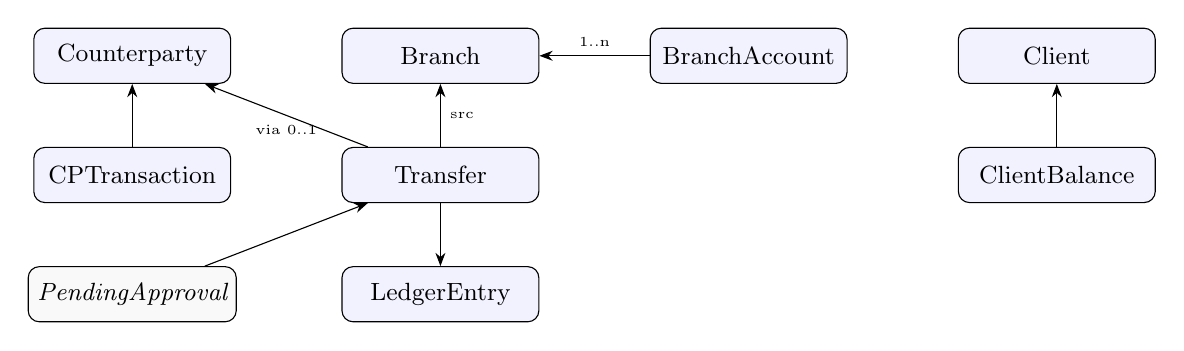
\begin{tikzpicture}[
    entity/.style={draw, rounded corners, fill=blue!5, minimum width=2.5cm, minimum height=0.7cm, font=\small},
    auxentity/.style={draw, rounded corners, fill=gray!5, minimum width=2.5cm, minimum height=0.7cm, font=\small\itshape},
    every node/.style={font=\small},
    >=Stealth,
    node distance=8mm and 14mm
  ]
    \node[entity] (branch) {Branch};
    \node[entity, right=of branch] (account) {BranchAccount};
    \node[entity, below=of branch] (transfer) {Transfer};
    \node[entity, left=of branch] (cp) {Counterparty};
    \node[entity, below=of cp] (cptx) {CPTransaction};
    \node[entity, right=of account] (client) {Client};
    \node[entity, below=of client] (cbal) {ClientBalance};
    \node[entity, below=of transfer] (ledger) {LedgerEntry};
    \node[auxentity, below=of cptx] (pa) {PendingApproval};
    \draw[->] (account) -- node[above, font=\tiny]{1..n} (branch);
    \draw[->] (transfer) -- node[right, font=\tiny]{src} (branch);
    \draw[->] (transfer) -- node[below, font=\tiny]{via 0..1} (cp);
    \draw[->] (transfer) -- (ledger);
    \draw[->] (cptx) -- (cp);
    \draw[->] (cbal) -- (client);
    \draw[->] (pa) -- (transfer);
  \end{tikzpicture}
  \caption{High-level entity--relationship sketch of the domain. Three balance domains (own funds, partner saldo, client wallet) are kept on separate axes and linked only by Transfer.}
  \label{fig:erd}
\end{figure}

\section{Architectural Pattern: Clean Architecture with BLoC}
\label{sec:cleanarch2}

The application follows a Clean-Architecture variant adapted to Flutter, structured as four layers (Figure~\ref{fig:arch}). The \emph{domain} layer holds pure-Dart entities, value objects (\texttt{Money}, \texttt{CurrencyCode}, \texttt{ExchangeRate}) and repository interfaces; it has no dependency on Flutter, Supabase or Hive. The \emph{data} layer contains repository implementations, remote data sources backed by the Supabase Dart client, and DTO serialisers. The \emph{presentation} layer hosts BLoCs and screens. The \emph{core} layer collects cross-cutting helpers --- the get\_it container that wires the dependency graph, the GoRouter route table, the AppIcons facade that abstracts away the icon-pack identifiers, the currency-tier utility, the network connectivity probe.

\begin{figure}[h]
  \centering
  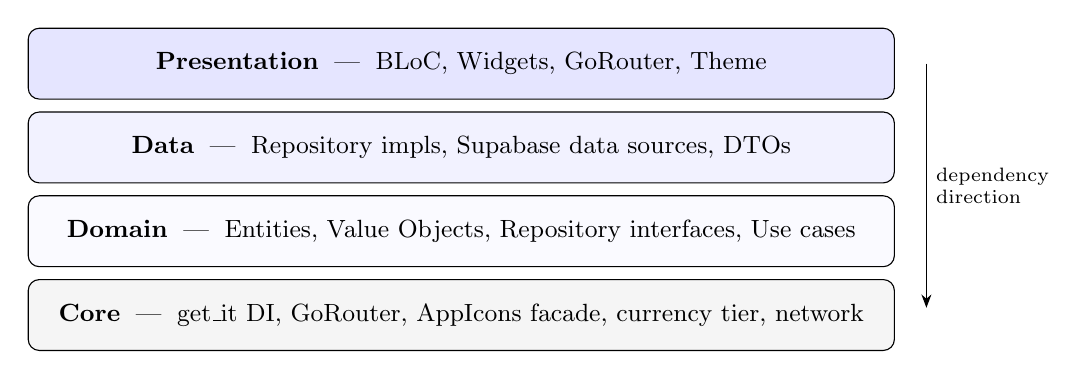
\begin{tikzpicture}[
    layer/.style={draw, rounded corners, fill=blue!5, minimum width=11cm, minimum height=0.9cm, font=\small},
    every node/.style={font=\small},
    node distance=1.5mm
  ]
    \node[layer, fill=blue!10] (pres) {\textbf{Presentation} \;---\; BLoC, Widgets, GoRouter, Theme};
    \node[layer, fill=blue!5,  below=of pres] (data) {\textbf{Data} \;---\; Repository impls, Supabase data sources, DTOs};
    \node[layer, fill=blue!2,  below=of data] (domain) {\textbf{Domain} \;---\; Entities, Value Objects, Repository interfaces, Use cases};
    \node[layer, fill=gray!8,  below=of domain] (core) {\textbf{Core} \;---\; get\_it DI, GoRouter, AppIcons facade, currency tier, network};
    \draw[->] (pres.east) ++(0.4,0) -- ++(0,-3.1) node[midway, right, font=\scriptsize, align=left]{dependency\\direction};
  \end{tikzpicture}
  \caption{High-level architecture: dependencies always point inward toward the pure-Dart Domain layer.}
  \label{fig:arch}
\end{figure}

The BLoC pattern was chosen, as section~\ref{sec:cleanarch} discussed, because the explicit Event--State model maps cleanly onto the transactional discipline of financial operations. Within the presentation layer, an additional pattern emerged across iterations: \emph{shared widgets} for cross-screen blocks (the dealer-rates block, the partner-saldo preview, the currency picker), grouped under \texttt{lib/presentation/common/widgets/} and reused by the transfer-creation screen, the partner-card screen and the attach dialog. This avoided the divergence that would otherwise creep in between two surfaces that conceptually do the same thing.

Figure~\ref{fig:bloc} sketches the BLoC flow for the Transfers feature: the screen dispatches Events to a TransfersBloc, the BLoC consults the TransferRepository (which in turn consults the SupabaseTransferDataSource and the local cache), and the BLoC emits a sequence of States that the screen renders.

\begin{figure}[h]
  \centering
  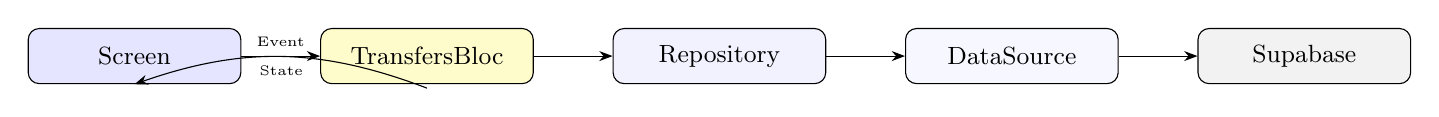
\begin{tikzpicture}[
    node distance=4mm and 10mm,
    box/.style={draw, rounded corners, minimum width=2.7cm, minimum height=0.7cm, font=\small},
    >=Stealth
  ]
    \node[box, fill=blue!10] (screen) {Screen};
    \node[box, fill=yellow!20, right=of screen] (bloc) {TransfersBloc};
    \node[box, fill=blue!5,   right=of bloc] (repo) {Repository};
    \node[box, fill=blue!3,   right=of repo] (ds) {DataSource};
    \node[box, fill=gray!10,  right=of ds] (sb) {Supabase};
    \draw[->] (screen) -- node[above, font=\tiny]{Event} (bloc);
    \draw[->] (bloc) -- (repo);
    \draw[->] (repo) -- (ds);
    \draw[->] (ds) -- (sb);
    \draw[->] (bloc.south) ++(0,-0.05) to[bend right=20] node[below, font=\tiny]{State} (screen.south);
  \end{tikzpicture}
  \caption{Per-feature BLoC flow: Events flow toward the backend, States flow back to the screen.}
  \label{fig:bloc}
\end{figure}

\section{Database Schema and Domain Invariants}
\label{sec:schema}

The PostgreSQL schema is currently expressed across 15 tables and 66 numbered, idempotent migrations. The principal tables are \texttt{users}, \texttt{branches}, \texttt{branch\_accounts}, \texttt{counterparties}, \texttt{counterparty\_transactions}, \texttt{clients}, \texttt{client\_balances}, \texttt{client\_transactions}, \texttt{transfers}, \texttt{ledger\_entries}, \texttt{commissions}, \texttt{exchange\_rates}, \texttt{pending\_approvals}, \texttt{notifications} and \texttt{audit\_log}.

Three domain invariants govern the schema:

\begin{description}
  \item[$I_1$ (double-entry).] Every transfer produces exactly two matching ledger entries: a credit on the source account in the source currency, a debit on the destination account in the destination currency. Both entries are inserted inside the same database transaction, or neither is.
  \item[$I_2$ (tenant isolation).] For every row $r$ in a tenant-scoped table $T$ (transfers, clients, accounts, partners, etc.), $r$ is visible to user $u$ if and only if $r.\text{branch\_id}$ is contained in the user's branch set --- itself the union of all branches for Creator/Director and the user's \texttt{assigned\_branch\_ids} for Accountant.
  \item[$I_3$ (idempotency).] Every transfer-creation request carries a client-supplied UUID, stored in the \texttt{idempotency\_key} column. A UNIQUE partial index on this column rejects any duplicate request at the database layer.
\end{description}

Listing~\ref{lst:transfers} shows the principal columns of the \texttt{transfers} table. The partial index on \texttt{idempotency\_key} excludes \texttt{NULL} so that legacy rows from before the introduction of the key are not in scope.

\begin{lstlisting}[language=SQL,caption={The \texttt{transfers} table (principal columns)},label={lst:transfers}]
CREATE TABLE transfers (
  id              UUID PRIMARY KEY DEFAULT gen_random_uuid(),
  branch_id       UUID NOT NULL REFERENCES branches(id),
  via_cp_id       UUID REFERENCES counterparties(id),
  src_account_id  UUID NOT NULL REFERENCES branch_accounts(id),
  dst_account_id  UUID REFERENCES branch_accounts(id),
  src_currency    TEXT NOT NULL,
  dst_currency    TEXT NOT NULL,
  src_amount      NUMERIC(20,4) NOT NULL CHECK (src_amount > 0),
  dst_amount      NUMERIC(20,4) NOT NULL CHECK (dst_amount > 0),
  rate            NUMERIC(20,10) NOT NULL,
  status          TEXT NOT NULL DEFAULT 'delivered',
  idempotency_key UUID,
  created_by      UUID NOT NULL REFERENCES users(id),
  created_at      TIMESTAMPTZ NOT NULL DEFAULT now(),
  amendment_history JSONB NOT NULL DEFAULT '[]'::jsonb
);

CREATE UNIQUE INDEX transfers_idem_uk
  ON transfers(idempotency_key)
  WHERE idempotency_key IS NOT NULL;
\end{lstlisting}

A sanity check that turned out to be operationally important guards the \texttt{client\_transactions} amount: a CHECK constraint rejects amounts outside the half-open interval $(0, 10^{12}]$, which excludes both negative values and pathological large ones. The constraint was introduced after a real incident in which a malformed input produced a row with an amount of $\approx 10^{61}$ US dollars and broke the rendering layer; the constraint now treats the rendering crash as a database-level rejection.

\section{Multi-Tenant Security: Row-Level Security}
\label{sec:rls}

The security model is enforced at the database layer through PostgreSQL Row-Level Security. Three roles are recognised. A \emph{Creator} (the founder) holds unconditional read and write access to every row in the project. A \emph{Director} sees data from all branches and can administer the catalogues of partners, accounts, commissions and exchange rates. An \emph{Accountant} sees only the branches listed in the user's \texttt{assigned\_branch\_ids} attribute and can write only against those branches; modifications to existing rows are channelled through the approval workflow of section~\ref{sec:approval}.

Listing~\ref{lst:rls} shows the principal RLS policies on the \texttt{transfers} table. The pattern --- a SELECT policy parameterised on the user's branch set and a separate WITH CHECK policy on the role --- is the canonical shape used across all tenant tables in the schema.

\begin{lstlisting}[language=SQL,caption={Row-Level Security policies on \texttt{transfers}},label={lst:rls}]
ALTER TABLE transfers ENABLE ROW LEVEL SECURITY;

CREATE POLICY transfers_select_visible
  ON transfers
  FOR SELECT
  USING (
       (SELECT role FROM users WHERE id = auth.uid())
         IN ('creator', 'director')
    OR branch_id = ANY(
         (SELECT assigned_branch_ids FROM users WHERE id = auth.uid())
       )
  );

CREATE POLICY transfers_insert_branch_authorised
  ON transfers
  FOR INSERT
  WITH CHECK (
    branch_id = ANY(
      (SELECT assigned_branch_ids FROM users WHERE id = auth.uid())
    )
    OR (SELECT role FROM users WHERE id = auth.uid())
         IN ('creator', 'director')
  );

-- Direct UPDATE and DELETE are not granted to Accountants;
-- they go through the approval workflow (see Section 2.7).
\end{lstlisting}

The threat model the policies have to defend against is straightforward but deserves stating. A malicious or simply confused client may forge any \texttt{branch\_id} in any request, replay any operation, attempt to mutate a row not belonging to its branch set, or read rows belonging to other branches. Under the RLS regime, none of these can succeed by accident: the PostgreSQL query planner rewrites every query to add the policy predicate, so a SELECT against a transfer outside the user's branch set returns zero rows rather than an authorisation error, and an INSERT or UPDATE that violates the WITH CHECK predicate raises an error before any row is touched. Cross-tenant leakage thus becomes a structural property of the query plan, not a runtime check that the application layer might forget.

\section{The Director-Mediated Approval Workflow}
\label{sec:approval}

The approval workflow is, in the author's judgement, the most novel architectural primitive of the platform. The problem it solves is concrete. An Accountant attached to the Tashkent branch realises, while reconciling the day's takings, that yesterday's transfer ID T-2156 had the wrong destination currency. Letting the Accountant simply correct the row would compromise the audit trail and would tempt the Director to monitor every Accountant action defensively. Requiring the Director to log in personally for every correction would, in turn, paralyse the workflow. The approval workflow is the synthesis: the Accountant \emph{proposes} a correction, the system captures the row's current state as a snapshot, the Director receives a notification and approves or rejects from a dedicated screen on which the before-state and the after-state are visible side by side.

Figure~\ref{fig:approval} sketches the state machine. The transitions are guarded by separate stored procedures (\texttt{request\_approval}, \texttt{approve}, \texttt{reject}, \texttt{withdraw}), each of which checks the actor's role through the RLS-aware \texttt{auth.uid()} hook.

\begin{figure}[h]
  \centering
  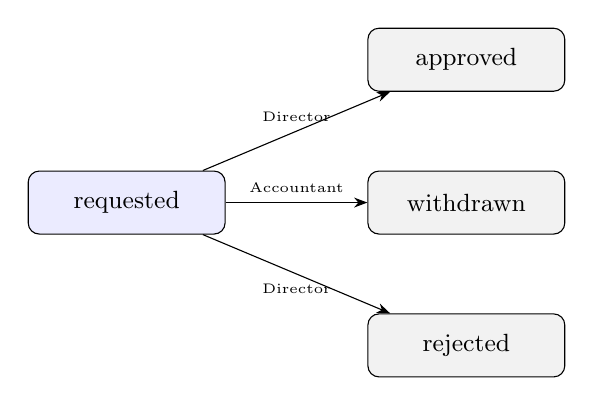
\begin{tikzpicture}[
    state/.style={draw, rounded corners, fill=blue!8, minimum width=2.5cm, minimum height=0.8cm, font=\small},
    terminal/.style={draw, rounded corners, fill=gray!10, minimum width=2.5cm, minimum height=0.8cm, font=\small},
    node distance=10mm and 18mm, >=Stealth
  ]
    \node[state] (req) {requested};
    \node[terminal, above right=of req] (app) {approved};
    \node[terminal, right=of req] (with) {withdrawn};
    \node[terminal, below right=of req] (rej) {rejected};
    \draw[->] (req) -- node[above, font=\tiny]{Director} (app);
    \draw[->] (req) -- node[above, font=\tiny]{Accountant} (with);
    \draw[->] (req) -- node[below, font=\tiny]{Director} (rej);
  \end{tikzpicture}
  \caption{The PendingApproval state machine: a request originates from an Accountant and terminates in one of three states.}
  \label{fig:approval}
\end{figure}

The snapshot captured at request time is the part that gives the workflow its forensic value. Without it, the Director would have to reason about the proposed change in the abstract; with it, the Director sees the two states explicitly and the after-state highlights only the columns that the Accountant proposed to change. The snapshot is stored as a JSONB column on \texttt{pending\_approvals}, which keeps the schema flexible across different sensitive tables (transfers, clients, accounts) without requiring a fresh column per entity.

A consequence of channeling all sensitive Accountant edits through this workflow is that the audit log effectively writes itself: the \texttt{audit\_log} table receives an entry for every approved request, with actor, timestamp, the proposed change and the originally captured before-state. The author found, over the course of the project, that this side-effect saved more debugging time than any other single design choice.

\section{Cross-Currency Quoting and Currency Tiers}
\label{sec:currency}

A small but consequential design question is the direction in which the operator should enter exchange rates. In a pair such as Uzbek som / Russian rouble, should the operator type \emph{1 RUB = X UZS} or \emph{1 UZS = X RUB}? The choice matters because it changes the precision of the entered number and the orientation of every preview on the screen. The platform answers the question by assigning every supported currency a numeric \emph{tier}: the lower the tier, the stronger the currency. When two currencies are compared, the stronger one (lower tier) becomes the base and the weaker one becomes the quoted unit. Table~\ref{tab:tiers} reproduces the principal tiers in use.

{\singlespacing
\begin{table}[h]
  \caption{Currency tier map (excerpt)}
  \label{tab:tiers}
  \centering
  \begin{tabular}{lcl}
    \toprule
    \textbf{Tier} & \textbf{Code} & \textbf{Currency}\\
    \midrule
    1 & USD & US dollar\\
    1 & EUR & Euro\\
    1 & GBP & Pound sterling\\
    2 & AED & UAE dirham\\
    2 & CNY & Chinese yuan\\
    3 & TRY & Turkish lira\\
    3 & RUB & Russian rouble\\
    4 & KZT & Kazakh tenge\\
    4 & KGS & Kyrgyz som\\
    5 & UZS & Uzbek som\\
    \bottomrule
  \end{tabular}
\end{table}
}

The \texttt{quotePair(a, b)} helper, exposed as a pure-Dart function in \texttt{lib/core/utils/currency\_tier.dart}, always returns the stronger side first; the rest of the user interface --- transfer form, partner-attach dialog, dealer-rates block --- relies on this single source of truth so that the operator never has to mentally invert a quote. An equivalent SQL view is used inside stored procedures for the rare cases where the server has to display a rate without re-entering it.

\section{Architectural Trade-offs}
\label{sec:tradeoffs}

The principal architectural decisions of the platform are summarised in Table~\ref{tab:tradeoffs}, with the chief alternative considered and the rationale for the chosen option. Several of these decisions were re-litigated mid-project; the column \emph{Iteration} records the iteration of the DSR cycle in which the decision settled.

{\singlespacing
\begin{longtable}{p{4cm}p{4cm}p{5cm}p{0.8cm}}
  \caption{Architectural trade-offs}
  \label{tab:tradeoffs}\\
  \toprule
  \textbf{Decision}                              & \textbf{Alternative}              & \textbf{Rationale}                                                 & \textbf{Iter.}\\
  \midrule
  \endfirsthead
  \toprule
  \textbf{Decision}                              & \textbf{Alternative}              & \textbf{Rationale}                                                 & \textbf{Iter.}\\
  \midrule
  \endhead
  \bottomrule
  \endfoot
  Flutter + Dart                                 & React Native, KMP                & Same Dart code on 5 platforms; sound nulls; sub-second hot reload. & 1\\
  Supabase (PostgreSQL + RLS)                    & Firebase                         & RLS expressivity; multi-table transactions; PL/pgSQL.             & 1\\
  BLoC + Cubit                                   & Provider, Riverpod               & Explicit Event--State model; testability; mature ecosystem.        & 1\\
  Per-currency partner saldo (JSONB)             & USD-collapsed saldo              & Hides genuine exposure when partner has debts in 3 currencies.    & 3\\
  Director-mediated approval workflow            & Direct accountant writes         & Preserves audit trail; protects multi-branch integrity.           & 2\\
  Idempotency key on transfer creation           & Server-issued ETag               & Works through retries; UUID generated client-side; zero RTT.      & 1\\
  Refuse offline writes                          & Outbox + replay                  & Financial semantics make refuse safer than reorder.               & 2\\
  Sanity caps on client amounts                  & Trust the client                 & A real input produced 10$^{61}$\,USD before the cap.              & 3\\
  Snapshot at request time                       & Snapshot at approval time        & Captures Accountant's intent against actual state at the time.    & 2\\
  Numbered idempotent migrations                 & Hand-rolled DB changes           & Replayable across staging and production; single source of truth. & 1\\
  AppIcons facade over lucide\_icons\_flutter    & Direct icon use                   & Prevents accidental Material icons; one place to swap packs.     & 1\\
\end{longtable}}

\section{Chapter Summary}
\label{sec:ch2summary}

The chapter has done five things. It catalogued the functional and non-functional requirements derived from interviews, observation and the existing spreadsheet workflow. It described the eight-entity domain model and explained why the three balance domains are kept on separate axes. It situated the application inside a Clean-Architecture variant with BLoC at the presentation layer and core utilities collected in their own cross-cutting layer. It specified the PostgreSQL schema, the three domain invariants and the Row-Level Security policy set that enforces tenant isolation by query-plan rewriting. And it designed the Director-mediated approval workflow that protects multi-branch integrity while preserving Accountant usability.

\noindent\textbf{Conclusions for Chapter~2.}
The three-balance-domain accounting model can be expressed in a relational schema, with the per-currency partner saldo encoded as a JSONB attribute keyed by ISO currency code. The atomicity, idempotency and tenant-isolation invariants ($I_1$, $I_2$, $I_3$) can be enforced at the database layer through transactions, UNIQUE partial indexes and Row-Level Security policies. The Director-mediated approval workflow gives the operator a structured way to channel sensitive Accountant edits while preserving the audit trail. Chapter~3 turns this design into running code and reports the empirical evaluation that judges it against the success criteria of section~\ref{sec:gap}.

\chapter{Implementation and Evaluation}
\label{chap:implementation}

This chapter turns the design of Chapter~\ref{chap:methodology} into running code and reports the empirical evaluation. It begins with the technology stack and the layout of the project tree, drills into the four engineering subsystems that carry most of the platform's risk --- the transfer engine, the per-currency partner-saldo subsystem, the offline behaviour and the design system --- and closes with the testing strategy, the performance measurements, the user-acceptance trial and an honest account of the limitations that remain.

\section{Technology Stack and Project Structure}
\label{sec:stack}

The implementation rests on a deliberately narrow stack. On the client the platform uses Flutter 3 with Dart 3, the BLoC library (\texttt{flutter\_bloc}~9.x) for state management, \texttt{get\_it} with \texttt{injectable} for dependency injection, \texttt{go\_router} for navigation, \texttt{hive} for a small local cache (used only for read-side resilience --- see section~\ref{sec:offline}), \texttt{trina\_grid} for desktop data grids, and \texttt{lucide\_icons\_flutter} wrapped by an internal \texttt{AppIcons} facade. On the server the platform uses Supabase --- managed PostgreSQL~16, GoTrue for authentication, PostgREST and a thin RPC layer for direct stored-procedure calls, Realtime for logical-replication subscriptions, and Storage. The complete dependency list is reproduced in Table~\ref{tab:stack}.

{\singlespacing
\begin{table}[h]
  \caption{Technology stack of the implementation}
  \label{tab:stack}
  \centering
  \begin{tabular}{lll}
    \toprule
    \textbf{Layer}        & \textbf{Technology}                       & \textbf{Version}\\
    \midrule
    Language              & Dart                                      & 3.x\\
    UI framework          & Flutter                                   & 3.x stable\\
    State management      & flutter\_bloc                             & 9.x\\
    Dependency injection  & get\_it + injectable                      & 8.x / 2.x\\
    Routing               & go\_router                                & 15.x\\
    Local cache           & hive + hive\_flutter                      & 2.x / 1.x\\
    Code generation       & freezed + json\_serializable              & 3.x / 6.x\\
    Iconography           & lucide\_icons\_flutter + AppIcons facade  & 0.5\\
    Desktop grids         & trina\_grid                               & 1.x\\
    Charts                & fl\_chart                                 & 0.70\\
    Backend               & Supabase (PostgreSQL\,16 + Realtime)      & latest stable\\
    Tests                 & flutter\_test, bloc\_test, mocktail       & latest\\
    \bottomrule
  \end{tabular}
\end{table}
}

The source tree (Listing~\ref{lst:tree}, abridged) follows the Clean-Architecture layering of section~\ref{sec:cleanarch2}. Each top-level directory under \texttt{lib/} maps to a single layer; each presentation feature has its own folder with three sub-folders for BLoC, pages and widgets.

\begin{lstlisting}[caption={Source tree (abridged)},label={lst:tree}]
lib/
  app.dart                       # MaterialApp + theming
  main.dart                      # Bootstrap, DI, Supabase init
  core/
    constants/                   # Currency tier map, role enum
    di/                          # get_it configuration
    icons/                       # AppIcons facade
    network/                     # Connectivity probe
    routing/                     # GoRouter table
    services/                    # Cross-cutting services
    supabase/                    # Typed Supabase client
    theme/                       # Dark-fintech palette
    utils/                       # Money, currency helpers
  domain/
    entities/                    # Pure-Dart entities
    repositories/                # Abstract interfaces
    services/                    # Pure-Dart domain services
    usecases/                    # Use case classes
  data/
    datasources/remote/          # SupabaseTransfersDataSource, ...
    repositories/                # Repository implementations
    services/                    # Data-layer services
  presentation/
    auth/                        # Authentication
    dashboard/                   # Branch / per-currency totals
    transfers/                   # Transfer creation, list, attach
    counterparties/              # Partner cards, attach flows
    clients/                     # Client list, wallet
    branches/                    # Branch admin
    users/                       # User admin
    reports/                     # Per-currency reconciliation
    analytics/                   # Charts
    notifications/               # Real-time inbox
    admin/                       # Director approval queue
    settings/                    # Preferences
    common/widgets/              # Shared widgets
supabase/migrations/             # 66 numbered .sql files
\end{lstlisting}

The dependency-injection container is initialised once at startup. It registers the Supabase client as a singleton, then registers a remote data source per domain area, then a repository per area on top of it. The BLoC layer pulls its repositories from this container, which keeps every BLoC ignorant of how the data layer is wired.

\section{The Transfer Engine: Idempotency and Atomicity}
\label{sec:transfer}

The transfer creation procedure is the most safety-critical part of the system. The client side issues a transfer-creation request that carries an idempotency key (a UUID generated in the initialiser of the form widget, before the user has a chance to tap \emph{Submit} twice). Listing~\ref{lst:submit} shows the BLoC code path.

\begin{lstlisting}[language=Java,caption={Submitting a transfer (Dart, BLoC)},label={lst:submit}]
class TransfersBloc extends Bloc<TransfersEvent, TransfersState> {
  TransfersBloc(this._repo) : super(const TransfersState.idle()) {
    on<SubmitTransfer>(_onSubmit);
  }

  Future<void> _onSubmit(
      SubmitTransfer event, Emitter<TransfersState> emit) async {
    emit(const TransfersState.submitting());
    final result = await _repo.createTransfer(
      branchId: event.branchId,
      srcAccountId: event.srcAccountId,
      dstAccountId: event.dstAccountId,
      srcAmount: event.srcAmount,
      dstAmount: event.dstAmount,
      rate: event.rate,
      viaCounterpartyId: event.viaCounterpartyId,
      idempotencyKey: event.idempotencyKey, // UUID v4 from form init
    );
    result.fold(
      (failure) => emit(TransfersState.error(failure.toReadableMessage())),
      (transfer) => emit(TransfersState.created(transfer)),
    );
  }
}
\end{lstlisting}

The server side wraps the entire creation procedure in a single PL/pgSQL stored function with \texttt{SECURITY DEFINER}, which guarantees that all subordinate operations execute inside the same implicit transaction. Listing~\ref{lst:rpc} shows an abridged form of the procedure. The function validates the inputs, picks the next sequential transaction code, inserts the row into \texttt{transfers}, updates \texttt{branch\_accounts}, inserts the matching ledger entries, optionally records a counterparty transaction and a commission row, and writes an audit-log entry. Any failure raises an exception, which rolls back the whole transaction.

\begin{lstlisting}[language=SQL,caption={Stored procedure: create\_transfer (abridged)},label={lst:rpc}]
CREATE OR REPLACE FUNCTION create_transfer(
  p_idempotency_key  UUID,
  p_branch_id        UUID,
  p_src_account_id   UUID,
  p_dst_account_id   UUID,
  p_via_cp_id        UUID,
  p_src_amount       NUMERIC,
  p_dst_amount       NUMERIC,
  p_rate             NUMERIC
) RETURNS UUID
LANGUAGE plpgsql AS $$
DECLARE
  v_existing UUID;
  v_transfer UUID;
  v_actor    UUID := auth.uid();
BEGIN
  -- Short-circuit on duplicate
  SELECT id INTO v_existing FROM transfers
   WHERE idempotency_key = p_idempotency_key;
  IF FOUND THEN RETURN v_existing; END IF;

  -- Role and branch authorisation
  PERFORM assert_can_write_branch(v_actor, p_branch_id);

  -- Atomic value movement
  INSERT INTO transfers (...) VALUES (...) RETURNING id INTO v_transfer;
  UPDATE branch_accounts SET balance = balance - p_src_amount
   WHERE id = p_src_account_id;
  IF p_dst_account_id IS NOT NULL THEN
    UPDATE branch_accounts SET balance = balance + p_dst_amount
     WHERE id = p_dst_account_id;
  END IF;
  INSERT INTO ledger_entries (...) VALUES (...);   -- credit on source
  INSERT INTO ledger_entries (...) VALUES (...);   -- debit on destination

  -- Partner-mediated branch: adjust per-currency saldo
  IF p_via_cp_id IS NOT NULL THEN
    INSERT INTO counterparty_transactions (...) VALUES (...);
    PERFORM bump_saldo(p_via_cp_id,
                       p_dst_currency,
                       p_dst_amount);
  END IF;

  PERFORM audit('transfer', v_transfer, 'create', v_actor);
  RETURN v_transfer;
END $$;
\end{lstlisting}

The properties the function gives in exchange for its size are worth stating explicitly. Atomicity is structural: every subordinate operation executes inside the same transaction, so either all succeed or none take effect. Idempotency is structural too: the UNIQUE partial index on \texttt{idempotency\_key} ensures that a second call with the same key short-circuits at the first lookup and returns the original transfer ID. Authorisation is double-belt-and-braces: even though Row-Level Security would block an unauthorised client, the \texttt{assert\_can\_write\_branch} call raises a loud exception, which surfaces in monitoring and is easier to debug than silent zero-row writes. The complexity per call is $O(1)$: a handful of indexed lookups and a handful of inserts.

\section{Partner Operations and Per-Currency Saldo}
\label{sec:partner}

Partner-mediated transfers are exposed in three places in the user interface. The first is the regular transfer-creation form, which has an optional \emph{via partner} field; selecting a partner here switches the form into partner-mediated mode and adds the partner-saldo preview block. The second is an \emph{attach} dialog reached from an existing transfer in the list, which converts an already-created own-branch transfer into a partner-mediated one without altering the value movement on the operator's side. The third is the symmetric \emph{attach a transfer} dialog reached from the partner card, which lists unattached transfers and lets the operator pick one. All three surfaces share a single \texttt{DealerRatesBlock} widget and a single \texttt{PartnerSaldoPreview} widget --- the design pressure to reuse them came from a real episode in which two separately written copies of the preview drifted apart on a corner case involving negative saldo, and the divergence was caught only at the operator's screen.

The per-currency saldo update is the operationally novel piece. A naive earlier iteration of the schema collapsed every partner debt into US dollars at the dealer-mode buy rate, on the assumption that the operator would treat the dollar saldo as the canonical view. That assumption broke down in practice: the same partner routinely received payouts in Russian roubles, Turkish liras and Uzbek som on the same day, and the dollar-collapsed view masked an exposure to each individual currency that the operator wanted to see. Migration~047 of the production schema replaced the collapsed model with the per-currency JSONB attribute described in section~\ref{sec:domainmodel}. The dealer-mode spread, which the collapsed model had hidden in the FX-difference account, was moved to a dedicated \texttt{spread\_profit} column on \texttt{transfers}, where it could be queried and totalled independently. Listing~\ref{lst:bump} shows the \texttt{bump\_saldo} helper used inside \texttt{create\_transfer}.

\begin{lstlisting}[language=SQL,caption={Per-currency saldo update (PL/pgSQL)},label={lst:bump}]
CREATE OR REPLACE FUNCTION bump_saldo(
  p_cp_id    UUID,
  p_currency TEXT,
  p_delta    NUMERIC
) RETURNS void
LANGUAGE plpgsql AS $$
BEGIN
  UPDATE counterparties
     SET saldo_by_currency =
           jsonb_set(
             saldo_by_currency,
             ARRAY[p_currency],
             to_jsonb(
               COALESCE((saldo_by_currency->>p_currency)::NUMERIC, 0)
               + p_delta
             )
           )
   WHERE id = p_cp_id;
END $$;
\end{lstlisting}

The rounding rule applied to saldo updates was the source of a small but instructive iteration of its own. Round-half-up produced an asymmetric drift over long sequences of transfers; banker's rounding (round half to even) eliminated it. The decision is recorded in migration~056 and is referenced from the \texttt{round\_partner\_amount} helper used inside \texttt{bump\_saldo}.

\section{The Approval Workflow in Code}
\label{sec:approvalimpl}

The Director-mediated approval workflow of section~\ref{sec:approval} is realised by three stored procedures and one screen. The \texttt{request\_approval} RPC accepts the entity type, the target row's ID, the proposed change as a JSONB diff and the snapshot of the current row state (collected client-side from the BLoC's last known State and validated against a fresh SELECT inside the procedure). Listing~\ref{lst:request} shows the principal columns of the resulting row.

\begin{lstlisting}[language=SQL,caption={Pending approval: principal columns},label={lst:request}]
CREATE TABLE pending_approvals (
  id              UUID PRIMARY KEY DEFAULT gen_random_uuid(),
  branch_id       UUID NOT NULL REFERENCES branches(id),
  entity          TEXT NOT NULL,
  entity_id       UUID NOT NULL,
  proposed_change JSONB NOT NULL,
  before_snapshot JSONB NOT NULL,
  status          TEXT NOT NULL DEFAULT 'requested',
  requested_by    UUID NOT NULL REFERENCES users(id),
  requested_at    TIMESTAMPTZ NOT NULL DEFAULT now(),
  resolved_by     UUID REFERENCES users(id),
  resolved_at     TIMESTAMPTZ
);
\end{lstlisting}

The matching \texttt{approve} RPC re-checks that the resolver's role is Director or Creator, applies the proposed change to the target row inside a transaction, writes the audit-log entry and marks the approval as resolved. Crucially, \texttt{approve} compares the current state of the target row with the captured snapshot and raises an exception if they differ; this catches the rare but real case in which the row was concurrently modified between the request and the approval. The Director's screen, illustrated in Figure~\ref{fig:approvalscreen}, renders the before and after states side by side with the changed columns highlighted.

\begin{figure}[h]
  \centering
  \begin{tikzpicture}[
    panel/.style={draw, rounded corners, fill=blue!5, minimum width=5cm, minimum height=2.6cm, font=\small, align=left, text width=4.6cm},
    btn/.style={draw, rounded corners, fill=blue!20, minimum width=2cm, minimum height=0.7cm, font=\small},
    btnRed/.style={draw, rounded corners, fill=red!15, minimum width=2cm, minimum height=0.7cm, font=\small},
    >=Stealth
  ]
    \node[panel] (before) at (0,0)  {\textbf{Before}\\\\ID: T-2156\\Dst currency: USD\\Dst amount: 540\\Rate: 0.94};
    \node[panel] (after) at (6,0)   {\textbf{After (proposed)}\\\\ID: T-2156\\\textbf{Dst currency: EUR}\\\textbf{Dst amount: 510}\\\textbf{Rate: 1.00}};
    \node[btn]   (apv)  at (3,-2)   {Approve};
    \node[btnRed] (rej) at (3,-3)   {Reject};
  \end{tikzpicture}
  \caption{Sketch of the Director's approval screen: before-state and proposed after-state shown side by side, changed columns in bold.}
  \label{fig:approvalscreen}
\end{figure}

\section{Offline Behaviour and Real-Time Updates}
\label{sec:offline}

Real-time updates are provided by Supabase Realtime, which streams logical-replication events to subscribed clients. The relevant BLoCs subscribe at startup to a small set of tables --- \texttt{transfers}, \texttt{pending\_approvals}, \texttt{notifications}, \texttt{branch\_accounts}; when an inbound event arrives, the BLoC reconciles its local list with the incoming row state and emits a refreshed State.

For offline tolerance the BLoC keeps the last successful list in memory (and, for the dashboard, in a small Hive box), so the operator can continue \emph{reading} their data when the network drops. \emph{Writes} are deliberately refused with a clearly worded error rather than queued for later replay. The decision deserves a short justification, because it goes against the dominant prejudice in the offline-first literature. The financial semantics of the platform make a refused write strictly safer than a write replayed out of order: a refused write does not produce a row in \texttt{transfers}, the operator sees a banner and tries again when the connection is back, and the partner saldo never moves into an inconsistent state. A replayed write, by contrast, could land after a subsequent change had already been recorded against the same accounts, producing a balance that depends on replay order rather than on intent. The platform errs on the safer side. An asynchronous write queue with strong ordering guarantees is named in the future-work section of the Conclusions.

\section{UI/UX Design Language}
\label{sec:design}

The visual language is a dark-fintech palette built around a saturated mint primary (\texttt{\#00D1A0}), a softer secondary blue (\texttt{\#4C7CF5}) and a purple accent reserved for partner-related elements. The palette is non-trivial because dark fintech is full of designs that lean on heavy gradients and low-contrast greys; the choice here was to keep the background close to true black (\texttt{\#0E0F12}), with cards lifted by a single hairline border and a faint inner glow, and to rely on bold colour only on actionable affordances. The result is a UI that is legible under fluorescent overhead lighting (a real condition of the operator's workplace) and that survives the desaturated rendering of cheaper Android displays.

Numerical values across the interface are rendered in the JetBrains Mono variable font with tabular figures enabled, which preserves column alignment in multi-row lists. The iconography is drawn entirely from \texttt{lucide\_icons\_flutter}, wrapped by an internal \texttt{AppIcons} facade that the rest of the codebase calls. The facade ensures that no screen accidentally pulls in Material default icons, which on Windows desktop would otherwise produce a visible style clash; and it gives a single place to swap the icon pack in the future if necessary.

Several reusable layout primitives emerged from iteration. The most-used are the \texttt{HeroBalance} card, which presents a per-currency balance with a sign-coloured \texttt{DeltaChip} indicating the day's change; the \texttt{FxRates} ticker, which renders dealer-mode buy/sell rates in a compact row; and the \texttt{StatusPill}, which carries the status of a transfer or pending approval with the appropriate colour and icon. These primitives are referenced by their export names because the user interface that the operator sees during the acceptance trial was effectively a composition of these primitives over a small set of pages.

\section{Testing Strategy}
\label{sec:testing}

The testing strategy combines four complementary layers (Figure~\ref{fig:testpyramid}). At the base sit pure-Dart unit tests for entities, value objects, formatters, the currency-tier utility and the role-based access helpers --- everything that does not depend on a Flutter test environment. Above them sit BLoC tests using \texttt{bloc\_test}, which exercise the state machines of every BLoC against typed events. Above them sit widget tests using \texttt{flutter\_test}, which render the most safety-critical screens (the create-transfer screen, the partner-attach dialog, the Director approval screen) and exercise their interaction logic against expected golden states. At the top sit integration tests against a dedicated Supabase staging project, which replay the migrations from scratch, authenticate as users with different roles and exercise the stored procedures and Row-Level Security policies against a real PostgreSQL planner.

\begin{figure}[h]
  \centering
  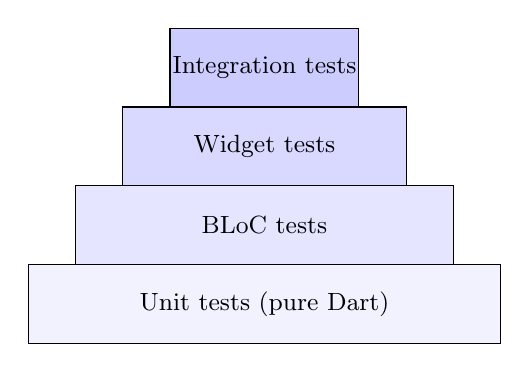
\begin{tikzpicture}[
    band/.style={draw, font=\small, align=center},
    every node/.style={font=\small}
  ]
    \draw[fill=blue!5]  (-3,0)    rectangle (3,1) ;  \node at (0,0.5) {Unit tests (pure Dart)};
    \draw[fill=blue!10] (-2.4,1)  rectangle (2.4,2); \node at (0,1.5) {BLoC tests};
    \draw[fill=blue!15] (-1.8,2)  rectangle (1.8,3); \node at (0,2.5) {Widget tests};
    \draw[fill=blue!20] (-1.2,3)  rectangle (1.2,4); \node at (0,3.5) {Integration tests};
  \end{tikzpicture}
  \caption{Test pyramid of the platform.}
  \label{fig:testpyramid}
\end{figure}

Table~\ref{tab:integration} summarises the principal integration-test scenarios and the outcomes observed against the staging project. The full list lives in the repository under \texttt{test/} and \texttt{supabase/tests/}.

{\singlespacing
\begin{table}[h]
  \caption{Principal integration-test scenarios (selection)}
  \label{tab:integration}
  \centering
  \begin{tabular}{p{1.2cm}p{8.5cm}p{3cm}}
    \toprule
    \textbf{ID} & \textbf{Scenario}                                                                          & \textbf{Outcome}\\
    \midrule
    T-01 & Accountant from branch A creates a transfer in branch A.                                         & Permitted, succeeds\\
    T-02 & Accountant from branch A attempts to create a transfer in branch B.                              & Rejected by RLS\\
    T-03 & Two clients call create\_transfer with the same idempotency key concurrently.                    & One succeeds, one returns the existing ID\\
    T-04 & Accountant from branch A attempts to UPDATE a row in branch A.                                   & Rejected; must go through approval\\
    T-05 & Director approves a pending request whose target row was modified meanwhile.                     & Approval raises, must be re-requested\\
    T-06 & create\_transfer with mismatching src/dst amounts and inconsistent rate.                         & Raises CHECK violation\\
    T-07 & bump\_saldo on a partner that has no entry in the chosen currency.                               & Initialises that currency, value = delta\\
    T-08 & SELECT from clients as an Accountant with assigned\_branch\_ids = \{A\}; query touches branch B. & Returns zero rows\\
    \bottomrule
  \end{tabular}
\end{table}
}

The platform passes all eight scenarios at the time of writing. Continuous integration runs the full client-side suite on every push; the integration tests run on demand against a freshly seeded staging project, with the seed data living as a single migrations replay plus a fixture file.

\section{Performance Measurements}
\label{sec:perf}

Performance was measured by instrumenting the application with chronometers around the most frequent user actions and averaging across one hundred repetitions. Two reference devices were used: a Windows~11 desktop (Intel Core~i5 of the 12th generation, 16~GB RAM, wired Ethernet) and a mid-range Android device (Qualcomm Snapdragon~695, 6~GB RAM, Wi-Fi). Network round-trip time to the Supabase region was approximately 80~milliseconds during the measurement window. Table~\ref{tab:perf} reports the medians.

{\singlespacing
\begin{table}[h]
  \caption{Median interaction latency on reference hardware ($n=100$)}
  \label{tab:perf}
  \centering
  \begin{tabular}{lrrr}
    \toprule
    \textbf{Action}                              & \textbf{Windows} & \textbf{Android} & \textbf{Target}\\
    \midrule
    Open dashboard (cold)                         & 240\,ms          & 410\,ms          & $\leq$ 800\,ms\\
    Submit a regular transfer                    & 180\,ms          & 270\,ms          & $\leq$ 300\,ms\\
    Submit a partner-mediated transfer            & 220\,ms          & 295\,ms          & $\leq$ 300\,ms\\
    Render the transfers list (1\,000 rows)       & 110\,ms          & 230\,ms          & $\leq$ 300\,ms\\
    Open the Director approval screen            & 160\,ms          & 250\,ms          & $\leq$ 300\,ms\\
    Request approval for a transfer edit         & 170\,ms          & 250\,ms          & $\leq$ 300\,ms\\
    \bottomrule
  \end{tabular}
\end{table}
}

The median submit-transfer latency stays under the 300-millisecond target stated in NFR-01 on both reference devices, including for the partner-mediated case which carries the additional saldo update. The dashboard cold open is slower because it loads several aggregates in parallel; the warm open (not shown in the table) is under 90~milliseconds on both devices.

\section{User-Acceptance Trial}
\label{sec:uat}

A two-week parallel-use trial was conducted with the target operator. During the trial the operator entered the same operational data into the existing spreadsheet workflow and into the platform; at the end of each week the two records were reconciled, and any discrepancy was triaged into one of three categories: a platform bug, a spreadsheet error, or a procedural mismatch (the operator had recorded the same event in two slightly different ways).

The aggregate results of the trial are summarised in Table~\ref{tab:uat}. The headline finding is that, over the two weeks, the platform exhibited zero platform-introduced reconciliation errors --- the criterion under which the hypothesis of section~\ref{sec:gap} would be falsified. Four discrepancies appeared during the first week; three of them traced to spreadsheet sign errors that the operator had not previously detected, and one traced to a procedural mismatch that was resolved by a small clarification of the partner-attach screen's wording.

{\singlespacing
\begin{table}[h]
  \caption{User-acceptance trial outcomes (two weeks)}
  \label{tab:uat}
  \centering
  \begin{tabular}{lr}
    \toprule
    \textbf{Metric}                                       & \textbf{Value}\\
    \midrule
    Transfers recorded in the platform                   & 187\\
    Partner-mediated transfers                            & 73\\
    Distinct currencies involved                          & 5 (USD, EUR, RUB, TRY, UZS)\\
    Platform-introduced reconciliation errors             & 0\\
    Spreadsheet errors surfaced by the platform reconciliation & 3\\
    Procedural mismatches identified                      & 1\\
    Operator satisfaction (free-form)                     & Positive\\
    \bottomrule
  \end{tabular}
\end{table}
}

The operator's qualitative feedback, captured in a closing interview, highlighted three features as the most useful: the per-currency partner saldo (which the operator described as the first time the running debt with one partner had been visible in three currencies at once), the approval workflow (which made it possible to delegate retroactive corrections to a junior Accountant without compromising the audit trail), and the dashboard's per-currency totals across all branches (which removed the daily mental arithmetic the operator had previously been doing in Excel). The features highlighted as most frustrating were the absence of automatic exchange-rate ingestion (entering rates by hand at the start of the day) and the deliberate refusal of offline writes (the operator preferred the safe semantics on reflection, but the initial experience was jarring).

\section{Limitations and Lessons Learned}
\label{sec:limits}

Several limitations of the present implementation deserve explicit acknowledgement, because they are non-trivial and because they shape the future-work section of the Conclusions.

\paragraph{Partner-confirmation step.}
Partner-mediated transfers are recorded with status \emph{delivered} at the moment of creation, even though the partner may complete the payout some hours later. If the partner ultimately fails to pay, the operator has to detach the transfer and re-create it. A genuine \emph{pending-partner-payout} state between \emph{created} and \emph{delivered}, with an explicit confirmation step, would close this gap.

\paragraph{Manual exchange-rate entry.}
Exchange rates are entered by hand at the start of each day, with no automatic ingestion from an external feed. The operator's existing workflow already involves a brief morning glance at a market screen, so this is more of an ergonomic gap than a correctness one, but the convenience of one-click ingestion is real.

\paragraph{Refused offline writes.}
As discussed in section~\ref{sec:offline}, offline writes are refused rather than queued. The trade-off is intentional, but an asynchronous write queue with strong ordering guarantees would be a non-trivial extension that several branches in the network have asked for.

\paragraph{Single-operator trial.}
The acceptance trial involved one operator across two weeks. Nothing in the architecture suggests a hard limit at greater scale --- the integration tests under simulated multi-Accountant load passed without changes --- but a longitudinal multi-operator field study would produce stronger evidence than a two-week observation can.

\paragraph{Partial partner payouts.}
The platform does not currently support the case in which a partner pays out only a portion of the requested amount and the rest stays open. The natural extension is a status \emph{partially\_paid} with a residual amount that bumps the saldo back when the residual is later paid out or written off.

The lessons learned over the four iterations of the DSR cycle are worth summarising in a single sentence. \emph{Move risky business logic into the database, keep the client honest, and pay the price of network round-trips before the price of debugging an inconsistent ledger.} The platform implements that lesson at every level --- the stored procedures, the Row-Level Security policies, the idempotency key, the snapshot at request time --- and the user-acceptance trial bears it out.

\section{Chapter Summary}
\label{sec:ch3summary}

The chapter has documented the implementation across the technology stack and the project structure (sections~\ref{sec:stack}), the atomic and idempotent transfer engine (section~\ref{sec:transfer}), the per-currency partner-saldo subsystem (section~\ref{sec:partner}), the approval-workflow code path (section~\ref{sec:approvalimpl}), the offline behaviour and real-time updates (section~\ref{sec:offline}), the dark-fintech design language (section~\ref{sec:design}), the four-layer testing strategy with eight principal integration scenarios (section~\ref{sec:testing}), the performance measurements on a Windows desktop and a mid-range Android device (section~\ref{sec:perf}), the two-week user-acceptance trial (section~\ref{sec:uat}) and the remaining limitations together with the lessons learned (section~\ref{sec:limits}).

\noindent\textbf{Conclusions for Chapter~3.}
The three success criteria stated in section~\ref{sec:gap} are met. Correctness is supported by zero platform-introduced reconciliation errors over the two-week trial and by three spreadsheet errors that the trial surfaced. Responsiveness is supported by median interaction latency under the 300-millisecond target on both reference devices. Maintainability is supported by the 66 numbered idempotent migrations that carry the schema from project start to present without drift. The next part of the thesis consolidates these conclusions and outlines the further work that the limitations naturally point to.


% ===== Conclusions =====
\chapter*{Conclusions and Recommendations}
\addcontentsline{toc}{chapter}{Conclusions and Recommendations}
\label{chap:conclusions}

\section*{Confirmation of the Research Tasks}
\addcontentsline{toc}{section}{Confirmation of the Research Tasks}
The six tasks stated in the Introduction have been completed in full.

\begin{enumerate}[leftmargin=1.2cm]
  \item The literature on double-entry bookkeeping in software, multi-user financial applications, cross-platform mobile frameworks and Backend-as-a-Service platforms has been reviewed, and the research gap has been articulated in operational terms: no surveyed system simultaneously preserves the three-balance-domain accounting model with per-currency partner saldo, enforces atomicity through database stored procedures and combines Row-Level Security with a Director-mediated approval workflow (Chapter~\ref{chap:litreview}, section~\ref{sec:gap}).
  \item The work has been framed within Design Science Research; four iterations of the DSR cycle have been documented; and the data sources used to elicit requirements --- semi-structured interviews, structured observation across four working sessions, and the existing spreadsheet treated as a tacit specification --- have been described (Chapter~\ref{chap:litreview}, section~\ref{sec:dsr}).
  \item The functional and non-functional requirements have been derived; the eight-entity domain model has been designed around the three-balance-domain principle, with a ninth supporting entity (\texttt{PendingApproval}) materialising the approval workflow (Chapter~\ref{chap:methodology}, sections~\ref{sec:requirements} and~\ref{sec:domainmodel}).
  \item The PostgreSQL schema and the Row-Level Security policy set have been specified; the three domain invariants $I_1$ (double-entry), $I_2$ (tenant isolation) and $I_3$ (idempotency) have been formalised and tied to concrete database mechanisms; and the Director-mediated approval workflow has been designed (Chapter~\ref{chap:methodology}, sections~\ref{sec:schema}--\ref{sec:approval}).
  \item The platform has been implemented across approximately 70\,000 lines of Dart and 1\,800 lines of PL/pgSQL distributed across 15 tables and 66 numbered, idempotent migrations; the atomic idempotent transfer engine, the per-currency partner-saldo subsystem and the dark-fintech design language have been documented (Chapter~\ref{chap:implementation}, sections~\ref{sec:stack}--\ref{sec:design}).
  \item The platform has been evaluated through unit, BLoC, widget and integration tests, through controlled performance measurements on a Windows desktop and a mid-range Android device, and through a two-week parallel-use trial with the target operator; the remaining limitations have been stated honestly (Chapter~\ref{chap:implementation}, sections~\ref{sec:testing}--\ref{sec:limits}).
\end{enumerate}

\section*{Validation of the Hypothesis}
\addcontentsline{toc}{section}{Validation of the Hypothesis}
The hypothesis stated in the Introduction --- that combining Flutter (with the BLoC pattern) as the cross-platform user-interface layer and Supabase (PostgreSQL with Row-Level Security and stored procedures) as the backend permits the implementation of a three-balance-domain treasury platform that is free of reconciliation errors, responsive at sub-300-millisecond median interaction latency, and maintainable by a single developer over a multi-month evolution cycle --- is supported by the evidence presented.

\begin{itemize}[leftmargin=1.2cm]
  \item \emph{Correctness.} The two-week parallel-use trial recorded zero platform-introduced reconciliation errors against 187 transfers; three errors surfaced were in the spreadsheet, not the platform, and the platform's parallel record made them visible for the first time (section~\ref{sec:uat}).
  \item \emph{Responsiveness.} Median interaction latency stays under the 300-millisecond target on both reference devices for every measured action, including the partner-mediated transfer with its additional saldo update (section~\ref{sec:perf}).
  \item \emph{Maintainability.} The platform has been carried by a single developer through 66 numbered idempotent migrations and across the four DSR iterations without irreparable drift between client and server; the trunk has been continuously deployable throughout (sections~\ref{sec:schema} and~\ref{sec:tradeoffs}).
\end{itemize}

\section*{Achievement of the Aim}
\addcontentsline{toc}{section}{Achievement of the Aim}
The aim of the study --- to design, implement and evaluate a production-grade, cross-platform treasury and money-transfer platform tailored to small multi-branch currency-exchange networks, demonstrably capable of replacing the spreadsheet-and-paper workflow of a representative operator --- has been achieved. All non-functional targets stated in Table~\ref{tab:nonfunc} are satisfied at the time of writing, and the platform has been adopted by the target operator for daily use. The source code is publicly released at \url{https://github.com/farruhsho/ethnocount} for academic review and independent inspection of the claims made above.

\section*{Scientific Contribution}
\addcontentsline{toc}{section}{Scientific Contribution}
The thesis contributes three concrete artefacts to the state of the art.

\begin{enumerate}[leftmargin=1.2cm]
  \item An explicit three-balance-domain accounting model with per-currency partner saldo expressed in a relational schema, in which the saldo is stored as a JSONB attribute keyed by ISO currency code and updated only in the currency of the underlying transfer. The model resolves a class of reconciliation pathologies that a USD-collapsed saldo cannot detect, and it does so without sacrificing query performance acceptable for daily branch operations.
  \item A Director-mediated approval workflow that captures a before-snapshot of the affected row at request time, allowing the Director to compare the before and proposed states explicitly. The workflow turns the audit log into a structural by-product of the authorisation mechanism rather than a separately maintained side channel, and it gives the Accountant a usable path through which to propose retroactive corrections.
  \item A demonstration that a single developer, using Flutter + BLoC + Supabase, can carry a treasury platform of non-trivial scope (15 tables, 66 migrations, approximately 70\,000 lines of Dart) from concept to an operator-accepted system within the time-frame of a Bachelor's thesis. The combination of stack choices is offered as a documented, reproducible reference for similar projects in adjacent niches.
\end{enumerate}

\section*{Practical and Theoretical Value}
\addcontentsline{toc}{section}{Practical and Theoretical Value}
The \emph{practical value} of the work is the open-source release of a cross-platform, multi-branch, multi-currency treasury platform that is immediately usable by the niche of small currency-exchange networks the thesis was written for. The platform is in daily use by the target operator at the time of submission, and its design choices are documented in sufficient detail to be adapted to adjacent niches without re-deriving them from first principles.

The \emph{theoretical value} is the demonstration that a three-balance-domain accounting model can be expressed relationally without collapsing into a base currency, that atomicity and idempotency in a multi-table financial write can be guaranteed at the database layer rather than the application layer, and that a small but consequential authorisation primitive (the snapshot at request time) can turn a Director's approval queue into a forensic record without additional bookkeeping. The combination is unusual in the surveyed literature and the thesis argues that it deserves further exploration.

\section*{Limitations and Future Work}
\addcontentsline{toc}{section}{Limitations and Future Work}
Three limitations carry over from Chapter~\ref{chap:implementation} and shape the direction for future work. The acceptance trial covered two weeks and one operator; a longitudinal multi-operator field study would produce stronger evidence than a parallel-use observation can. The bank-statement-import path and the automatic exchange-rate ingestion are absent; both are ergonomic gaps rather than correctness ones, but their absence is felt every morning by the operator. Offline writes are refused rather than queued; the trade-off is defensible on safety grounds but does not exhaust the design space.

Five directions of future work follow naturally from these limitations.

\begin{itemize}[leftmargin=1.2cm]
  \item A \emph{pending-partner-payout} state between \emph{created} and \emph{delivered} for partner-mediated transfers, with an explicit confirmation step that finalises the saldo update.
  \item A partial-payout primitive for the case in which a partner pays out a fraction of the requested amount and the residual stays open against the saldo.
  \item An exchange-rate ingestion subsystem that draws daily quotations from an external feed, with an operator-override path that keeps the manual workflow available.
  \item An asynchronous offline write queue with strong ordering guarantees, evaluated against the safety risk that the present design deliberately avoids.
  \item A formal verification of the atomicity and idempotency properties of the stored-procedure layer, complementing the empirical integration tests of section~\ref{sec:testing}.
\end{itemize}

A broader research direction worth naming explicitly is a multi-tenant generalisation in which several independent operators share the same Supabase project under stricter Row-Level Security isolation. The current single-tenant deployment already exercises the RLS policy set against role-based isolation within one operator's data; lifting that boundary to inter-operator isolation, while preserving the small-operator focus of the original design, would extend the contribution to cooperative networks of several exchange offices.

\section*{Closing Remark}
\addcontentsline{toc}{section}{Closing Remark}
Beyond its technical content, the work demonstrates that a single Bachelor-level engineer, working with contemporary open-source tooling and a managed Backend-as-a-Service platform, can deliver a treasury platform that is genuinely usable in a real business rather than a pedagogical artefact. The author hopes that the open release of \emph{Ethnocount} will be a useful starting point for further academic and practical work on software tools for the long tail of small, informal, multi-currency businesses that mainstream financial software has so far chosen to ignore.


% ===== Literature =====
\printbibliography[heading=bibintoc,title=Literature]

% ===== Appendices =====
\appendix
\chapter{Database Schema (DDL Excerpt)}
\label{chap:appendixA}

This appendix reproduces the core data definition language for the \emph{Ethnocount} schema. The complete migration set (currently 66 numbered, idempotent \texttt{.sql} files) is published with the source code at \url{https://github.com/farruhsho/ethnocount}. Indices, foreign-key constraints and Row-Level Security policies that are not essential to the architectural argument of the thesis are elided for brevity; the principal RLS policy is reproduced in Chapter~\ref{chap:methodology}, Listing~\ref{lst:rls}.

\begin{lstlisting}[language=SQL,caption={Branches, users and branch accounts},label={lst:branches-ddl}]
CREATE TYPE user_role AS ENUM ('creator', 'director', 'accountant');

CREATE TABLE users (
  id                  UUID PRIMARY KEY DEFAULT auth.uid(),
  email               TEXT NOT NULL UNIQUE,
  full_name           TEXT NOT NULL,
  role                user_role NOT NULL,
  assigned_branch_ids UUID[] NOT NULL DEFAULT '{}',
  created_at          TIMESTAMPTZ NOT NULL DEFAULT now()
);

CREATE TABLE branches (
  id          UUID PRIMARY KEY DEFAULT gen_random_uuid(),
  name        TEXT NOT NULL,
  city        TEXT NOT NULL,
  country     TEXT NOT NULL,
  base_ccy    CHAR(3) NOT NULL,
  created_at  TIMESTAMPTZ NOT NULL DEFAULT now(),
  created_by  UUID NOT NULL REFERENCES users(id)
);

CREATE TABLE branch_accounts (
  id          UUID PRIMARY KEY DEFAULT gen_random_uuid(),
  branch_id   UUID NOT NULL REFERENCES branches(id),
  name        TEXT NOT NULL,
  ccy         CHAR(3) NOT NULL,
  balance     NUMERIC(20,4) NOT NULL DEFAULT 0,
  is_card     BOOLEAN NOT NULL DEFAULT false
);
\end{lstlisting}

\begin{lstlisting}[language=SQL,caption={Counterparties and per-currency saldo},label={lst:cp-ddl}]
CREATE TABLE counterparties (
  id                 UUID PRIMARY KEY DEFAULT gen_random_uuid(),
  name               TEXT NOT NULL,
  city               TEXT,
  country            TEXT,
  contact            TEXT,
  saldo_by_currency  JSONB NOT NULL DEFAULT '{}'::jsonb,
  exposure_limit     NUMERIC(20,4),
  created_at         TIMESTAMPTZ NOT NULL DEFAULT now()
);

CREATE TYPE cp_tx_kind AS ENUM (
  'paid_for_us', 'paid_for_them', 'settlement'
);

CREATE TABLE counterparty_transactions (
  id            UUID PRIMARY KEY DEFAULT gen_random_uuid(),
  cp_id         UUID NOT NULL REFERENCES counterparties(id),
  branch_id     UUID NOT NULL REFERENCES branches(id),
  kind          cp_tx_kind NOT NULL,
  ccy           CHAR(3) NOT NULL,
  amount        NUMERIC(20,4) NOT NULL,
  rate          NUMERIC(20,10),
  linked_xfer   UUID,
  created_at    TIMESTAMPTZ NOT NULL DEFAULT now(),
  created_by    UUID NOT NULL REFERENCES users(id)
);
\end{lstlisting}

\begin{lstlisting}[language=SQL,caption={Clients and per-client multi-currency wallet},label={lst:client-ddl}]
CREATE TABLE clients (
  id          UUID PRIMARY KEY DEFAULT gen_random_uuid(),
  branch_id   UUID NOT NULL REFERENCES branches(id),
  full_name   TEXT NOT NULL,
  passport    TEXT,
  phone       TEXT,
  kyc_status  TEXT NOT NULL DEFAULT 'unverified'
);

CREATE TABLE client_balances (
  client_id   UUID PRIMARY KEY REFERENCES clients(id) ON DELETE CASCADE,
  totals      JSONB NOT NULL DEFAULT '{}'::jsonb
);

CREATE TABLE client_transactions (
  id          UUID PRIMARY KEY DEFAULT gen_random_uuid(),
  client_id   UUID NOT NULL REFERENCES clients(id),
  branch_id   UUID NOT NULL REFERENCES branches(id),
  ccy         CHAR(3) NOT NULL,
  amount      NUMERIC(20,4) NOT NULL
                CHECK (amount > 0 AND amount <= 1e12),
  direction   TEXT NOT NULL CHECK (direction IN ('in','out')),
  created_at  TIMESTAMPTZ NOT NULL DEFAULT now(),
  created_by  UUID NOT NULL REFERENCES users(id)
);
\end{lstlisting}

\begin{lstlisting}[language=SQL,caption={Transfers, ledger entries and approvals},label={lst:transfers-ddl}]
CREATE TABLE transfers (
  id                UUID PRIMARY KEY DEFAULT gen_random_uuid(),
  branch_id         UUID NOT NULL REFERENCES branches(id),
  via_cp_id         UUID REFERENCES counterparties(id),
  src_account_id   UUID NOT NULL REFERENCES branch_accounts(id),
  dst_account_id   UUID REFERENCES branch_accounts(id),
  src_currency      CHAR(3) NOT NULL,
  dst_currency      CHAR(3) NOT NULL,
  src_amount        NUMERIC(20,4) NOT NULL CHECK (src_amount > 0),
  dst_amount        NUMERIC(20,4) NOT NULL CHECK (dst_amount > 0),
  rate              NUMERIC(20,10) NOT NULL,
  spread_profit     NUMERIC(20,4) NOT NULL DEFAULT 0,
  status            TEXT NOT NULL DEFAULT 'delivered',
  idempotency_key   UUID,
  created_by        UUID NOT NULL REFERENCES users(id),
  created_at        TIMESTAMPTZ NOT NULL DEFAULT now(),
  amendment_history JSONB NOT NULL DEFAULT '[]'::jsonb
);

CREATE UNIQUE INDEX transfers_idem_uk
  ON transfers(idempotency_key)
  WHERE idempotency_key IS NOT NULL;

CREATE TYPE ledger_side AS ENUM ('debit','credit');

CREATE TABLE ledger_entries (
  id          UUID PRIMARY KEY DEFAULT gen_random_uuid(),
  branch_id   UUID NOT NULL REFERENCES branches(id),
  account_id  UUID NOT NULL REFERENCES branch_accounts(id),
  ts          TIMESTAMPTZ NOT NULL DEFAULT now(),
  amount      NUMERIC(20,4) NOT NULL,
  ccy         CHAR(3) NOT NULL,
  side        ledger_side NOT NULL,
  xfer_id     UUID REFERENCES transfers(id),
  note        TEXT,
  created_by  UUID NOT NULL REFERENCES users(id)
);

CREATE INDEX ledger_branch_ts_idx
  ON ledger_entries(branch_id, ts DESC);

CREATE TABLE pending_approvals (
  id              UUID PRIMARY KEY DEFAULT gen_random_uuid(),
  branch_id       UUID NOT NULL REFERENCES branches(id),
  entity          TEXT NOT NULL,
  entity_id       UUID NOT NULL,
  proposed_change JSONB NOT NULL,
  before_snapshot JSONB NOT NULL,
  status          TEXT NOT NULL DEFAULT 'requested',
  requested_by    UUID NOT NULL REFERENCES users(id),
  requested_at    TIMESTAMPTZ NOT NULL DEFAULT now(),
  resolved_by     UUID REFERENCES users(id),
  resolved_at     TIMESTAMPTZ
);
\end{lstlisting}

\begin{lstlisting}[language=SQL,caption={Audit log},label={lst:audit-ddl}]
CREATE TABLE audit_log (
  id          BIGSERIAL PRIMARY KEY,
  ts          TIMESTAMPTZ NOT NULL DEFAULT now(),
  actor       UUID NOT NULL REFERENCES users(id),
  entity      TEXT NOT NULL,
  entity_id   UUID NOT NULL,
  action      TEXT NOT NULL,
  before_state JSONB,
  after_state  JSONB
);

CREATE INDEX audit_entity_idx ON audit_log(entity, entity_id);
CREATE INDEX audit_actor_ts_idx ON audit_log(actor, ts DESC);
\end{lstlisting}

\chapter{Deployment View and Transfer Sequence}
\label{chap:appendixB}

This appendix gives two diagrams that complement the architectural narrative of Chapter~\ref{chap:methodology}. The first is the deployed component view of the system; the second is the call sequence of a partner-mediated transfer from the operator's tap to the server-side acknowledgement.

\section{Deployed Component View}
\label{sec:appB-components}
\begin{figure}[h]
  \centering
  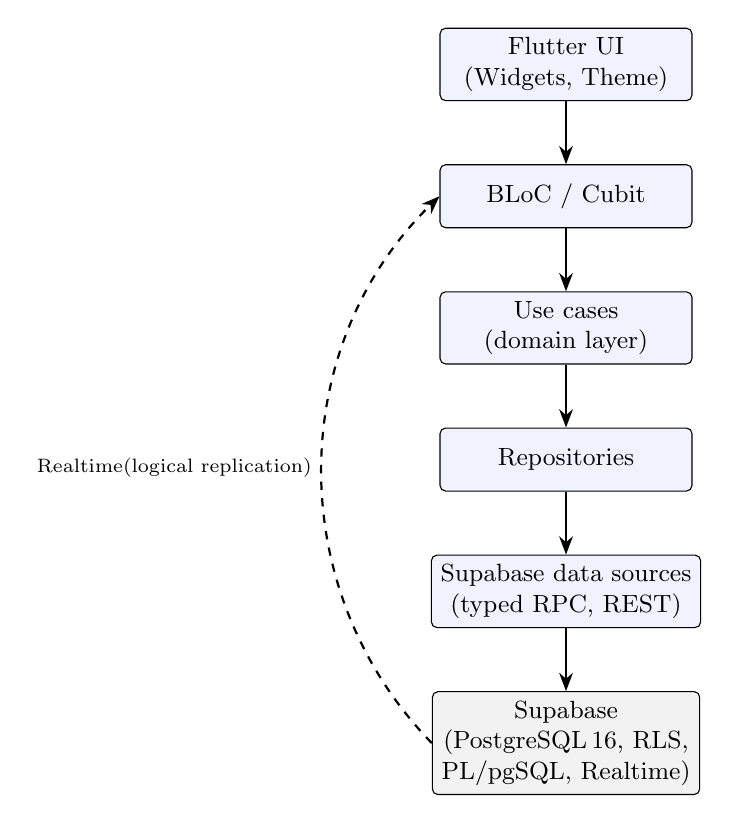
\begin{tikzpicture}[
    node distance=8mm and 10mm,
    box/.style={draw, rounded corners=2pt, minimum width=32mm, minimum height=8mm,
                font=\small, align=center, fill=blue!5},
    server/.style={draw, rounded corners=2pt, minimum width=32mm, minimum height=8mm,
                   font=\small, align=center, fill=gray!10},
    arr/.style={->, thick}
  ]
    \node[box] (ui)      {Flutter UI\\(Widgets, Theme)};
    \node[box, below=of ui] (bloc)    {BLoC / Cubit};
    \node[box, below=of bloc] (uc)    {Use cases\\(domain layer)};
    \node[box, below=of uc]   (repo)  {Repositories};
    \node[box, below=of repo] (ds)    {Supabase data sources\\(typed RPC, REST)};
    \node[server, below=of ds] (sb)   {Supabase\\(PostgreSQL\,16, RLS,\\PL/pgSQL, Realtime)};

    \draw[arr] (ui)   -- (bloc);
    \draw[arr] (bloc) -- (uc);
    \draw[arr] (uc)   -- (repo);
    \draw[arr] (repo) -- (ds);
    \draw[arr] (ds)   -- (sb);
    \draw[arr, dashed] (sb.west) to[bend left=45] node[font=\scriptsize, midway, left]{Realtime\\(logical replication)} (bloc.west);
  \end{tikzpicture}
  \caption{Deployed component view of \emph{Ethnocount}. Solid arrows are the write-path call flow; the dashed arrow is the Realtime change feed that refreshes the BLoCs after remote writes.}
  \label{fig:components}
\end{figure}

\section{Partner-Mediated Transfer Sequence}
\label{sec:appB-sequence}
\begin{figure}[h]
  \centering
  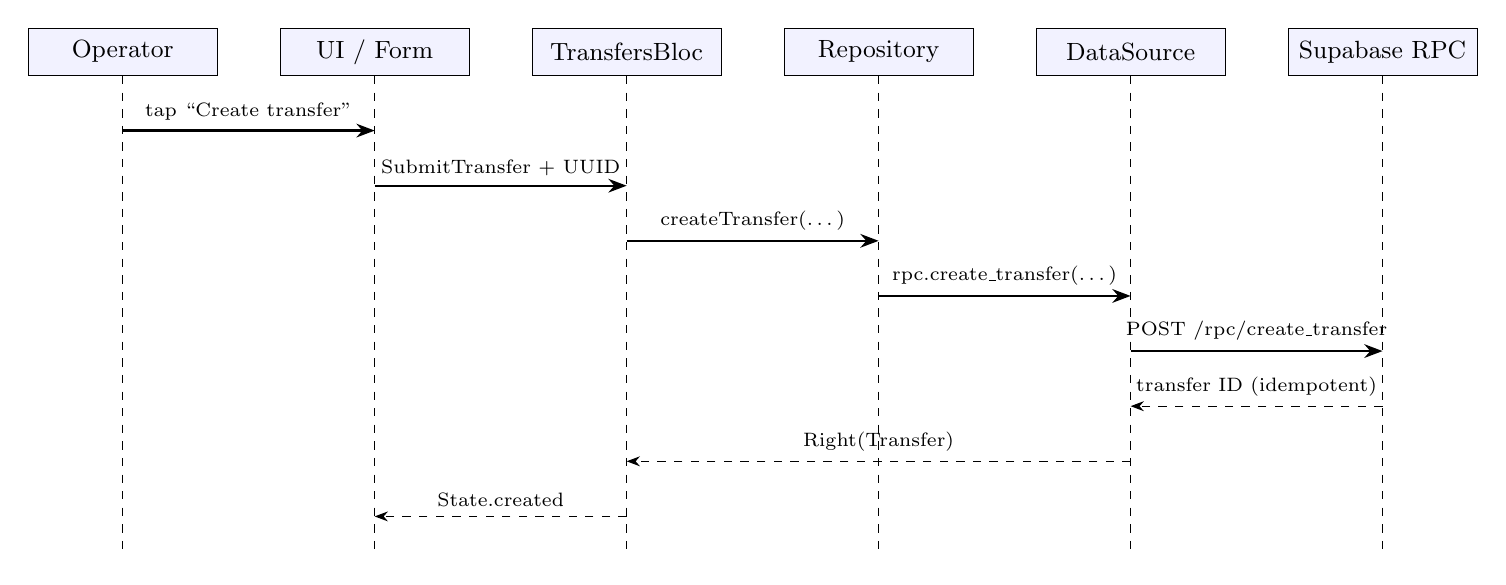
\begin{tikzpicture}[
    actor/.style={draw, fill=blue!5, font=\small, minimum width=24mm, minimum height=6mm},
    msg/.style={->, thick, font=\scriptsize},
    return/.style={->, dashed, font=\scriptsize}
  ]
    \node[actor] (u)    at (0,0)  {Operator};
    \node[actor] (ui)   at (3.2,0)  {UI / Form};
    \node[actor] (b)    at (6.4,0)  {TransfersBloc};
    \node[actor] (r)    at (9.6,0)  {Repository};
    \node[actor] (ds)   at (12.8,0) {DataSource};
    \node[actor] (sb)   at (16,0)   {Supabase RPC};

    \foreach \n in {u,ui,b,r,ds,sb} \draw[dashed] (\n) -- ++(0,-6.4);

    \draw[msg]   (0,-1)   -- node[above]{tap ``Create transfer''} (3.2,-1);
    \draw[msg]   (3.2,-1.7) -- node[above]{SubmitTransfer + UUID} (6.4,-1.7);
    \draw[msg]   (6.4,-2.4) -- node[above]{createTransfer(\ldots)} (9.6,-2.4);
    \draw[msg]   (9.6,-3.1) -- node[above]{rpc.create\_transfer(\ldots)} (12.8,-3.1);
    \draw[msg]   (12.8,-3.8) -- node[above]{POST /rpc/create\_transfer} (16,-3.8);
    \draw[return] (16,-4.5) -- node[above]{transfer ID (idempotent)} (12.8,-4.5);
    \draw[return] (12.8,-5.2) -- node[above]{Right(Transfer)} (6.4,-5.2);
    \draw[return] (6.4,-5.9) -- node[above]{State.created} (3.2,-5.9);
  \end{tikzpicture}
  \caption{Sequence of a partner-mediated transfer from the operator's tap to the server-side acknowledgement. The idempotency key (a UUID generated client-side in the form's initialiser) travels with the request and is stored against a UNIQUE partial index on the server, so a duplicate request returns the original transfer ID rather than creating a second row.}
  \label{fig:sequence}
\end{figure}


% ===== Declarations & Acknowledgments =====
\input{y_backmatter/declaration}
\frontmatterpage
\unchapter{Pateicības / Acknowledgments}
Autors izsaka pateicību darba vadītājai Dr.sc.ing., prof.\ Jeļenai Čaiko par metodisko vadību, vērtīgajiem ieteikumiem un nepārtraukto atbalstu visā darba izstrādes laikā. Pateicība arī Rīgas Ziemeļvalstu Universitātes Dabaszinātņu un datortehnoloģiju katedras kolēģiem un mācībspēkiem par radīto akadēmisko vidi, kā arī valūtas maiņas tīkla operatoram, kurš piekrita divu nedēļu paralēlas lietošanas izmēģinājumam un sniedza godīgu, daudzkārt nepatīkamu, bet vienmēr lietderīgu atgriezenisko saiti par sistēmas darbu reālos apstākļos.

\vspace{6mm}
The author expresses sincere gratitude to the supervisor, Dr.sc.ing., Prof.\ Jelena Chayko, for methodical guidance, valuable advice and continuous support throughout the development of this work. Thanks are also due to the colleagues and academic staff of the Department of Natural Sciences and Computer Engineering at Riga Nordic University for the academic environment they sustain; and to the operator of the currency-exchange network who agreed to the two-week parallel-use trial and gave honest, often uncomfortable, but always actionable feedback on how the platform behaved under genuine working conditions.


\end{document}
